% Core chapters. This file is included by the main textbook.
% Convention: actual minus ideal OPL; real, disk-RMS normalized Z_n^m.

\chapter{What a Zernike coefficient actually means}
\label{zc:meaning}

\section{From one number to a function of position}
A ruler can measure the height of one point on a mirror. It cannot describe the
whole mirror with that one measurement. A surface is a function: given two
coordinates, the function returns a height. Similarly, a wavefront error is a
function that returns an optical path difference at each pupil position. The
purpose of a Zernike expansion is to describe such a function using a sequence
of numbers, each multiplying a precisely defined spatial pattern.

The phrase ``Zernike constants'' usually means \emph{Zernike coefficients}.
They are constant with respect to position within one fitted map. They need
not remain constant when wavelength, field angle, temperature, focus,
illumination, aperture, alignment, or the reference surface changes. A mirror
does not possess one universal list of Zernike coefficients independent of
these choices.

Consider a circular pupil of physical radius $a$, centred at $(x_c,y_c)$.
Define dimensionless coordinates
\begin{equation}
 X=\frac{x-x_c}{a},\qquad Y=\frac{y-y_c}{a},\qquad
 \rho=\sqrt{X^2+Y^2},\qquad \theta=\operatorname{atan2}(Y,X).
 \label{zc:coordinates}
\end{equation}
The pupil is the disk $0\leq\rho\leq1$. Angle increases counterclockwise
from positive $X$ toward positive $Y$ when this coordinate plane is viewed
in the orientation used to define the map. Looking at a mirror from its
opposite side can reverse an axis. Therefore ``clockwise on the mirror''
is not sufficient metadata; label the actual coordinate axes.

Suppose, for example, that
\begin{equation}
 W(X,Y)=20\,\mathrm{nm}+30\,\mathrm{nm}\,X
                  +40\,\mathrm{nm}(X^2-Y^2).
\end{equation}
The numbers multiply functions, not points. At the centre the last two
terms vanish. At $(X,Y)=(1,0)$ the value is $90\,\mathrm{nm}$; at
$(0,1)$ it is $-20\,\mathrm{nm}$. A coefficient does not usually equal
the maximum error or the error at the pupil edge. Its meaning depends on
the scale chosen for its multiplying function.

\section{The distinction between a surface and a wavefront}
We will use three different quantities:
\begin{align}
 z(x,y)&:\quad\text{geometrical surface sag},\\
 h(x,y)&:\quad\text{surface departure from a specified nominal surface},\\
 W(x,y)&:\quad\text{actual optical eikonal minus ideal eikonal}.
\end{align}
All three may have length units, but they represent different objects.
An eikonal is optical path length accumulated with a specified phase
reference. At a common output plane, or on an explicitly chosen common
comparison surface,
\begin{equation}
 W=S_{\mathrm{actual}}-S_{\mathrm{ideal}},\qquad
 \phi=\frac{2\pi}{\lambda_0}W,
 \label{zc:opdconvention}
\end{equation}
where $\lambda_0$ is the vacuum wavelength and $\phi$ is the corresponding
phase difference in radians. Optical path includes refractive index:
$S=\int n\,ds$. A positive $W$ means that the actual phase, in the
$\exp(i k_0 S-i\omega t)$ convention, has accumulated more than the ideal
phase at the same comparison location.

A sag expansion is a geometrical prescription. A wavefront expansion is
an optical performance description relative to a chosen ideal wave.
Converting one to the other requires the incident field, reflection or
refraction law, pupil mapping, and reference wave. Near normal incidence
a small mirror height error produces twice the optical path error in
magnitude. A lens thickness error instead introduces an index difference.
We derive both statements later, including their signs and limitations.

\section{A basis is a set of building blocks}
In a plane, any vector can be written as $v_x\bm e_x+v_y\bm e_y$.
The unit vectors are building blocks, and $v_x,v_y$ are coordinates.
For functions, the building blocks are functions themselves:
\begin{equation}
 W(\rho,\theta)=\sum_{n,m}c_n^m Z_n^m(\rho,\theta).
 \label{zc:expansion}
\end{equation}
If the $Z_n^m$ are dimensionless, the coefficients $c_n^m$ have the units
of $W$. A coefficient of $0.05\,\mu\mathrm m$ is $50\,\mathrm{nm}$;
it is $0.10$ waves only when $\lambda_0=500\,\mathrm{nm}$.
The superscript $m$ is an index, not an exponent of the coefficient.

A finite polynomial expansion represents a finite-dimensional model of a
map. It does not assert that every manufactured error is polynomial.
Tool marks, scratches, discontinuities at segment boundaries, and
unresolved roughness can require many modes or a different representation.
A model is useful when its retained coefficients and its residual together
answer the design question.

\section{Averages over a disk and the area element}
A small polar patch has radial width $d\rho$ and tangential width
$\rho\,d\theta$, so its area is $\rho\,d\rho\,d\theta$. Define
\begin{equation}
 \langle f,g\rangle_D=
 \frac1\pi\int_0^{2\pi}\int_0^1
       f(\rho,\theta)g(\rho,\theta)\rho\,d\rho\,d\theta.
 \label{zc:innerproduct}
\end{equation}
The factor $1/\pi$ divides by the disk area. Thus $\langle1,1\rangle_D=1$.
For radial functions,
\begin{equation}
 \langle\rho^p,1\rangle_D=2\int_0^1\rho^{p+1}\,d\rho
                 =\frac{2}{p+2},\qquad p>-2.
 \label{zc:radialmoment}
\end{equation}
For example, the mean of $\rho^2$ is $1/2$, not $1/3$. The value $1/3$
comes from averaging uniformly in radius, which overweights the centre
relative to physical area. This distinction is central to numerical
sampling and least-squares fitting.

The mean is $\overline W=\langle W,1\rangle_D$. The standard deviation
of the wavefront, usually called its piston-removed RMS error, is
\begin{equation}
 \sigma_W=\sqrt{\langle W-\overline W,W-\overline W\rangle_D}.
 \label{zc:rmsdefinition}
\end{equation}
An unqualified ``RMS'' is ambiguous: $\sqrt{\langle W,W\rangle_D}$
includes piston, whereas Eq.~\eqref{zc:rmsdefinition} does not.
Piston changes the overall phase of a coherent beam but does not change
its isolated intensity image. Differential piston between subapertures
does change interference and cannot be discarded independently without
changing the optical system.

\section{Why orthogonality makes coefficients useful}
Two functions are orthogonal when their inner product is zero. They are
orthonormal when, additionally, each has unit squared norm. We will use
\begin{equation}
 \langle Z_n^m,Z_{n'}^{m'}\rangle_D
       =\delta_{nn'}\delta_{mm'},
 \label{zc:orthonormal}
\end{equation}
where a Kronecker delta is one for equal indices and zero otherwise.
Multiply Eq.~\eqref{zc:expansion} by $Z_{n'}^{m'}$ and integrate. Every
term vanishes except the matching one, giving
\begin{equation}
 \boxed{c_n^m=\langle W,Z_n^m\rangle_D.}
 \label{zc:projection}
\end{equation}
This is a projection formula: the coefficient measures the component of
the wavefront parallel to a particular function.

To see why projection is also the best least-squares approximation,
let $\widehat W=\sum_{j=1}^M c_j Z_j$ and minimize
$E=\langle W-\widehat W,W-\widehat W\rangle_D$. Differentiation gives
\begin{equation}
 \frac{\partial E}{\partial c_k}
  =-2\langle W,Z_k\rangle_D+2\sum_jc_j\langle Z_j,Z_k\rangle_D.
\end{equation}
For an orthonormal basis the sum is simply $2c_k$. Setting the derivative
to zero proves Eq.~\eqref{zc:projection}. The residual is orthogonal to
every retained mode. Therefore the error cannot be reduced by adding
another amount of a mode that has already been fitted.

Since the piston mode is $Z_0^0=1$, an expansion over the complete disk
has
\begin{equation}
 \overline W=c_0^0,\qquad
 \sigma_W^2=\sum_{(n,m)\ne(0,0)}(c_n^m)^2.
 \label{zc:parseval}
\end{equation}
For a truncated fit the squared norm of the remaining residual must also
be included to recover the total error. Equation~\eqref{zc:parseval} is
not generally valid on an annulus, an irregular mask, or a differently
weighted pupil when ordinary disk Zernikes are retained.

\chapter{Constructing Zernike polynomials from scratch}
\label{zc:construction}

\section{Why the angular functions are sines and cosines}
A point returns to itself when $\theta$ increases by $2\pi$; a physical
map must have the same value there. The functions $\cos(m\theta)$ and
$\sin(m\theta)$ satisfy this condition for integer $m$. They also have
particularly simple rotation laws and orthogonality:
\begin{align}
 \int_0^{2\pi}\cos(m\theta)\cos(m'\theta)\,d\theta
       &=\pi\delta_{mm'} &&(m,m'>0),\\
 \int_0^{2\pi}\sin(m\theta)\sin(m'\theta)\,d\theta
       &=\pi\delta_{mm'} &&(m,m'>0),\\
 \int_0^{2\pi}\sin(m\theta)\cos(m'\theta)\,d\theta&=0.
\end{align}
The constant angular function has squared integral $2\pi$ instead of
$\pi$. This factor of two will explain the different normalization of
rotationally symmetric and non-symmetric modes.

The number $|m|$ counts angular cycles around the pupil. It does not count
radial rings and does not by itself specify the degree of a polynomial.
For example, $\rho^2\cos2\theta=X^2-Y^2$ has two angular cycles and
degree two. The identity
\begin{equation}
 (X+iY)^\ell=\rho^\ell\bigl(\cos\ell\theta+i\sin\ell\theta\bigr)
\end{equation}
shows why a regular Cartesian polynomial with angular frequency $\ell$
begins with $\rho^\ell$. Multiplication by $\rho^2=X^2+Y^2$ preserves
that angular frequency. Thus the allowed radial powers are
$\rho^\ell,\rho^{\ell+2},\rho^{\ell+4},\ldots$.

\section{Gram--Schmidt: remove what has already been represented}
We first construct rotationally symmetric modes. Start with $1$ and
then $\rho^2$. Subtract the mean of the second:
\begin{equation}
 q_2=\rho^2-\langle\rho^2,1\rangle_D=\rho^2-\frac12.
\end{equation}
Its norm is
\begin{align}
 \langle q_2,q_2\rangle_D
 &=\langle\rho^4,1\rangle_D-\langle\rho^2,1\rangle_D+\frac14\\
 &=\frac13-\frac12+\frac14=\frac1{12}.
\end{align}
Division by $1/\sqrt{12}$ therefore gives
\begin{equation}
 Z_2^0=\sqrt3(2\rho^2-1).
 \label{zc:defocuspoly}
\end{equation}
This operation is Gram--Schmidt orthogonalization. Its physical meaning
here is that the new pattern contains no mean optical path.

Now start with $\rho^4$ and remove its projections onto $1$ and $Z_2^0$:
\begin{align}
 q_4&=\rho^4-\frac13
       -\langle\rho^4,Z_2^0\rangle_D Z_2^0,\\
 \langle\rho^4,Z_2^0\rangle_D
   &=\sqrt3\left(2\frac14-\frac13\right)=\frac{\sqrt3}{6},\\
 q_4&=\rho^4-\rho^2+\frac16.
\end{align}
Squaring this polynomial and using Eq.~\eqref{zc:radialmoment} gives
$\langle q_4,q_4\rangle_D=1/180$. Consequently,
\begin{equation}
 Z_4^0=\sqrt5(6\rho^4-6\rho^2+1).
 \label{zc:sphericalpoly}
\end{equation}
The lower powers are essential. A pure quartic term is not orthogonal
to piston or focus. The Zernike mode commonly called primary spherical
aberration already contains the lower-order terms that make it
orthogonal to both.

For a nonzero angular frequency, consider $\rho\cos\theta=X$.
Its mean square is $1/4$, so $Z_1^1=2\rho\cos\theta=2X$.
To construct a higher mode with the same angular frequency, begin with
$\rho^3\cos\theta$ and remove the tilt projection:
\begin{align}
 \langle\rho^3\cos\theta,2\rho\cos\theta\rangle_D
     &=2\int_0^1\rho^5\,d\rho=\frac13,\\
 q_3&=\left(\rho^3-\frac23\rho\right)\cos\theta.
\end{align}
Its squared norm is $1/72$. The normalized result is
\begin{equation}
 Z_3^1=\sqrt8(3\rho^3-2\rho)\cos\theta.
\end{equation}
This is balanced coma. The subtraction of a tilt term is mathematical
orthogonalization; it does not mean that a physical coma-producing
surface necessarily introduces an equal and opposite mechanical tilt.

\section{A general construction using one new variable}
Fix the nonnegative angular frequency $\ell=|m|$ and write
$n=\ell+2k$ with $k=0,1,2,\ldots$. Introduce $u=\rho^2$ and seek
\begin{equation}
 R_n^\ell(\rho)=\rho^\ell Q_k(u).
\end{equation}
The radial inner product becomes
\begin{equation}
 \int_0^1R_n^\ell R_{n'}^\ell\rho\,d\rho
   =\frac12\int_0^1u^\ell Q_k(u)Q_{k'}(u)\,du.
\end{equation}
We therefore need ordinary polynomials orthogonal on $[0,1]$ with
weight $u^\ell$. A convenient construction is
\begin{equation}
 \boxed{Q_k(u)=\frac1{k!u^\ell}
       \frac{d^k}{du^k}\left[u^{k+\ell}(u-1)^k\right].}
 \label{zc:rodrigues}
\end{equation}
The apparent division by $u^\ell$ does not produce a singular function:
each differentiated term still contains that power. This is a shifted
Jacobi Rodrigues formula; the general Jacobi conventions are documented
by NIST~\cite{zc:dlmfRodrigues}.

We can prove orthogonality without assuming any theory of special
functions. Let $p_j(u)$ be any polynomial of degree $j<k$. Substitute
Eq.~\eqref{zc:rodrigues}:
\begin{equation}
 \int_0^1u^\ell Q_k p_j\,du
 =\frac1{k!}\int_0^1p_j
        \frac{d^k}{du^k}\left[u^{k+\ell}(u-1)^k\right]du.
\end{equation}
Integrate by parts once. The derivative transfers to $p_j$, with a minus
sign. The boundary term vanishes because the bracket has a zero of
order at least $k$ at both endpoints. Repeat $k$ times. All boundary
terms vanish for the same reason, leaving
\begin{equation}
 \frac{(-1)^k}{k!}\int_0^1
       \frac{d^kp_j}{du^k}u^{k+\ell}(u-1)^k\,du=0.
\end{equation}
The last equality follows because the $k$th derivative of a polynomial
of degree less than $k$ is zero. Hence $Q_k$ is orthogonal to every
earlier polynomial, including $Q_0,\ldots,Q_{k-1}$.

\section{Deriving the normalization instead of memorizing it}
The leading coefficient of $Q_k$ is
\begin{equation}
 C_k=\frac{(2k+\ell)!}{k!(k+\ell)!}.
\end{equation}
Indeed, the highest term inside the derivative in
Eq.~\eqref{zc:rodrigues} is $u^{2k+\ell}$. After $k$ derivatives
and division by $k!u^\ell$, the displayed coefficient remains.
Using $p=Q_k$ in the integration-by-parts calculation now gives
\begin{align}
 \int_0^1u^\ell Q_k^2\,du
 &=\frac{(-1)^k}{k!}\int_0^1Q_k^{(k)}
                       u^{k+\ell}(u-1)^k\,du\\
 &=C_k\int_0^1u^{k+\ell}(1-u)^k\,du\\
 &=C_k\frac{(k+\ell)!k!}{(2k+\ell+1)!}
   =\frac1{2k+\ell+1}=\frac1{n+1}.
\end{align}
The factorial integral in the third line can itself be proved by
repeated integration by parts, starting with
$\int_0^1u^p\,du=1/(p+1)$. Returning to $\rho$ gives
\begin{equation}
 \int_0^1[R_n^\ell(\rho)]^2\rho\,d\rho=\frac1{2(n+1)}.
 \label{zc:radialnorm}
\end{equation}

Combining this result with the angular integrals leads to our complete
definition:
\begin{equation}
 \boxed{Z_n^m(\rho,\theta)=
 \begin{cases}
 \sqrt{n+1}\,R_n^0(\rho),&m=0,\\
 \sqrt{2(n+1)}\,R_n^m(\rho)\cos(m\theta),&m>0,\\
 \sqrt{2(n+1)}\,R_n^{|m|}(\rho)\sin(|m|\theta),&m<0.
 \end{cases}}
 \label{zc:definition}
\end{equation}
The allowed pairs obey $n\geq0$, $|m|\leq n$, and $n-|m|$ even.
Negative $m$ is our label for a sine, not an instruction to evaluate
$\sin(m\theta)$ with a negative argument. This distinction prevents an
otherwise easy sign error.

\section{The factorial formula and Jacobi connection}
Expand $(u-1)^k$ by the binomial theorem in
Eq.~\eqref{zc:rodrigues}, differentiate each power, and set $u=\rho^2$.
Relabelling the finite sum gives
\begin{equation}
 \boxed{R_n^\ell(\rho)=
 \sum_{s=0}^{(n-\ell)/2}
 \frac{(-1)^s(n-s)!}
 {s!\left(\frac{n+\ell}{2}-s\right)!
      \left(\frac{n-\ell}{2}-s\right)!}\rho^{n-2s}.}
 \label{zc:factorial}
\end{equation}
This formula is explicit and useful at low order. At high order the
individual terms can be enormous while their sum is small, so
floating-point cancellation becomes serious. Recurrences or stable
Jacobi evaluators are preferable for high radial degree.

In the standard Jacobi convention,
\begin{equation}
 R_{\ell+2k}^{\ell}(\rho)
       =\rho^\ell P_k^{(0,\ell)}(2\rho^2-1).
 \label{zc:jacobi}
\end{equation}
The substitution $x=2u-1$ converts the Jacobi weight
$(1-x)^0(1+x)^\ell$ into a constant multiple of $u^\ell$.
It also gives $R_n^\ell(1)=1$. Thus a library routine must be called
with parameters $(0,\ell)$ and argument $2\rho^2-1$ for this particular
identity. Swapping the parameters without also changing the argument
and sign gives a different polynomial.

\section{A complete radial table through degree six}
In Table~\ref{zc:radialtable}, each nonzero $\ell$ generates both a cosine
and a sine mode using Eq.~\eqref{zc:definition}. All modes through $n=6$
are therefore specified; there are $1+2+3+4+5+6+7=28$ real modes.
The descriptive names are aids to recognition, whereas $(n,m)$ and
the explicit formula define the function.

\begin{longtable}{@{}ccl@{}}
\caption{Radial polynomials through $n=6$.}\label{zc:radialtable}\\
\toprule
$n$&$\ell$&$R_n^\ell(\rho)$\\\midrule\endfirsthead
\toprule $n$&$\ell$&$R_n^\ell(\rho)$\\\midrule\endhead
0&0&$1$\\
1&1&$\rho$\\
2&0&$2\rho^2-1$\\
2&2&$\rho^2$\\
3&1&$3\rho^3-2\rho$\\
3&3&$\rho^3$\\
4&0&$6\rho^4-6\rho^2+1$\\
4&2&$4\rho^4-3\rho^2$\\
4&4&$\rho^4$\\
5&1&$10\rho^5-12\rho^3+3\rho$\\
5&3&$5\rho^5-4\rho^3$\\
5&5&$\rho^5$\\
6&0&$20\rho^6-30\rho^4+12\rho^2-1$\\
6&2&$15\rho^6-20\rho^4+6\rho^2$\\
6&4&$6\rho^6-5\rho^4$\\
6&6&$\rho^6$\\\bottomrule
\end{longtable}

For example,
\begin{align}
 Z_2^2&=\sqrt6(X^2-Y^2),&
 Z_2^{-2}&=2\sqrt6XY,\\
 Z_3^1&=\sqrt8[3(X^2+Y^2)-2]X,&
 Z_3^{-1}&=\sqrt8[3(X^2+Y^2)-2]Y,\\
 Z_3^3&=\sqrt8(X^3-3XY^2),&
 Z_3^{-3}&=\sqrt8(3X^2Y-Y^3).
\end{align}
Cartesian forms are useful when differentiating at the origin, where
polar-coordinate derivatives contain removable singular expressions.

\section{Single-index systems and the danger of a bare number}
Optical software often replaces $(n,m)$ by one index $j$. Noll,
OSA/ANSI, Fringe, and software-specific orderings do not all assign the
same functions to the same integer. They can also use different
normalizations or signs. Therefore a statement such as ``coefficient 8
is $0.2$'' is incomplete.

To exchange coefficients safely, export a table containing $n$, $m$,
the polynomial or normalization, units, aperture radius, coordinate
orientation, OPD sign, reference wave, and removed terms. To convert
from a function $F_j=\alpha_j Z_n^m$ carrying coefficient $b_j$, use
$c_n^m=\alpha_jb_j$ after matching the actual functions. If the other
package reverses the sine convention, the relevant $\alpha_j$ is
negative. Never infer a conversion solely from a familiar-looking
aberration name. The optical-metrology discussion by Wyant and Creath
also emphasizes convention and sampling issues~\cite{zc:wyant}.

\chapter{Reading a coefficient table as an optical diagnosis}
\label{zc:interpretation}

\section{Piston, tilt, and focus are choices as well as errors}
For a full disk, $c_0^0$ is the mean OPD. The next two modes are
$2X$ and $2Y$, representing a plane wave tilted relative to the reference.
Their physical gradients are
\begin{equation}
 \frac{\partial W_{\mathrm{tilt}}}{\partial x}=
 \frac{2c_1^1}{a},\qquad
 \frac{\partial W_{\mathrm{tilt}}}{\partial y}=
 \frac{2c_1^{-1}}{a}.
\end{equation}
At a forward output plane in medium $n'$, the paraxial ray direction
change is the gradient divided by $n'$. At a distance $L$ this gives
\begin{equation}
 \Delta x=\frac{2L}{n'a}c_1^1,\qquad
 \Delta y=\frac{2L}{n'a}c_1^{-1}.
 \label{zc:tiltshift}
\end{equation}
The sign is positive for the actual-minus-ideal convention: a positive
$x$ gradient increases the forward ray's $x$ direction cosine.
This follows from $\bm s=\nabla S/n'$; it should not be copied into a
different OPD convention without changing signs.

Defocus changes quadratic phase curvature. At an output plane $z=0$,
an ideal converging spherical wave whose centre is $(0,0,L)$ has, after
choosing zero phase at the pupil centre,
\begin{equation}
 S_{\mathrm{id},L}(r)=n'\left[L-\sqrt{L^2+r^2}\right]
           =-\frac{n'r^2}{2L}+\frac{n'r^4}{8L^3}+\cdots.
\end{equation}
Changing the reference focus to $L+\delta L$ gives
\begin{equation}
 S_{\mathrm{id},L+\delta L}-S_{\mathrm{id},L}
       \simeq\frac{n'r^2}{2L^2}\delta L.
\end{equation}
For fixed actual wavefront, the residual $W=S_{\mathrm{actual}}-S_{\mathrm{id}}$
therefore changes by the \emph{negative} of this quantity. Since
$r^2=a^2[1+Z_2^0/\sqrt3]/2$,
\begin{equation}
 \delta c_2^0=-\frac{n'a^2}{4\sqrt3L^2}\delta L,
 \qquad
 \delta L_{\mathrm{remove}}=
        \frac{4\sqrt3L^2}{n'a^2}c_2^0.
 \label{zc:focusshift}
\end{equation}
This is a small-shift, paraxial relation with the pupil held fixed. It
explains why removing defocus numerically corresponds approximately to
refocusing physically. Moving a detector or element in a real system
can also change pupil mapping and higher-order aberrations.

\section{Astigmatism and the orientation of a paired mode}
Let $a_c=c_2^2$ and $a_s=c_2^{-2}$. Then
\begin{equation}
 W_{\mathrm{ast}}=\sqrt6\rho^2
                 [a_c\cos2\theta+a_s\sin2\theta].
\end{equation}
Define $A=\sqrt{a_c^2+a_s^2}$ and
$\psi=\tfrac12\operatorname{atan2}(a_s,a_c)$. Using the cosine
subtraction identity gives
\begin{equation}
 W_{\mathrm{ast}}=\sqrt6A\rho^2\cos[2(\theta-\psi)].
\end{equation}
The orientation is ambiguous by $\pi$, as expected for an unoriented
principal axis. Exchanging which axis is called positive also changes
the sign representation. The quantity $A$ is the RMS contribution of
the pair on the full disk and is invariant under rotation.

Near the centre this wavefront has different quadratic curvatures along
its two principal axes. Rays in the two corresponding meridional planes
therefore focus at different axial distances. This explains the
association with astigmatism. At a single field point the coefficient
does not identify whether the cause was a tilted element, a cylindrical
surface error, system design, or stress.

\section{Coma, spherical aberration, and balanced polynomials}
The lowest coma pair has $n=3$, $|m|=1$. It has one angular cycle but
an additional radial structure compared with tilt. The primary spherical
mode has $n=4$, $m=0$. Higher radial members of these families are often
called secondary coma, secondary spherical aberration, and so forth.
These names identify pupil patterns at a fixed field point.

Classical aberration \emph{order} is a different bookkeeping system.
A quartic wavefront term has a cubic gradient and contributes to
third-order ray aberration. Moreover, a fourth-degree joint expansion
in pupil and field includes coma and astigmatism terms with lower
pupil degree. Thus Zernike radial degree $n$ is neither automatically
Seidel order nor ray order. The companion aberrations textbook develops
the joint pupil--field expansion explicitly.

The following exact algebraic identities translate common radial
monomials into our normalized modes:
\begin{align}
 \rho^2&=\frac12+\frac{Z_2^0}{2\sqrt3},\\
 \rho^4&=\frac13+\frac{Z_2^0}{2\sqrt3}
                        +\frac{Z_4^0}{6\sqrt5},\\
 \rho^6&=\frac14+\frac{9Z_2^0}{20\sqrt3}
                 +\frac{Z_4^0}{4\sqrt5}
                 +\frac{Z_6^0}{20\sqrt7}.
 \label{zc:monomialidentities}
\end{align}
For the last identity, solve
$R_6^0=20\rho^6-30\rho^4+12\rho^2-1$ for $\rho^6$, substitute the
preceding two identities, and collect coefficients. The resulting
constant is $1/4$, as independently required by the disk mean.

Consequently, if
\begin{equation}
 W=A\rho^4+B\rho^6+D\rho^2+C,
\end{equation}
then
\begin{align}
 c_0^0&=C+\frac D2+\frac A3+\frac B4,\\
 c_2^0&=\frac{D+A}{2\sqrt3}+\frac{9B}{20\sqrt3},\\
 c_4^0&=\frac A{6\sqrt5}+\frac B{4\sqrt5},\\
 c_6^0&=\frac B{20\sqrt7}.
 \label{zc:quarticsixth}
\end{align}
These equations are useful in design because a sixth-power sag or phase
term also changes lower radial Zernike coefficients. Controlling
$c_6^0$ independently generally requires compensating lower powers.

\section{A numerical coefficient budget}
Suppose the nonzero coefficients after removing piston, tilt, and focus
are $c_2^2=30\,\mathrm{nm}$, $c_2^{-2}=40\,\mathrm{nm}$,
$c_3^1=20\,\mathrm{nm}$, and $c_4^0=-10\,\mathrm{nm}$.
The astigmatism pair contributes $50\,\mathrm{nm}$ RMS, and the full
retained map has
\begin{equation}
 \sigma_W=\sqrt{30^2+40^2+20^2+(-10)^2}\,\mathrm{nm}
           =54.77\,\mathrm{nm}.
\end{equation}
The sign matters for the shape and for compensation, but not for the
individual squared contribution. At $\lambda_0=550\,\mathrm{nm}$ the
error is $0.0996$ waves RMS. If the unmodelled residual independently
orthogonal to the fitted modes has RMS $15\,\mathrm{nm}$, the total is
$\sqrt{3000+225}=56.79\,\mathrm{nm}$. Reporting only $54.77\,\mathrm{nm}$
would omit measured structure.

\chapter{Zernike coefficients of mirrors}
\label{zc:mirrors}

\section{Deriving the reflection factor with reference planes}
Consider a small planar mirror patch. Let its unit normal $\bm N$ point
into the incident medium. An incident ray has unit propagation direction
$\bm s_i$ with $\bm s_i\cdot\bm N=-\cos i$, where $i$ is measured
from the normal. Its reflected direction is
\begin{equation}
 \bm s_r=\bm s_i-2(\bm s_i\cdot\bm N)\bm N,
 \qquad \bm s_r\cdot\bm N=+\cos i.
\end{equation}
Move the reflecting patch by $h\bm N$, with $h>0$ toward the incident
medium. Keep the incident and outgoing phase-reference planes fixed.
The first-order change of the incoming optical path is
$n\bm s_i\cdot(h\bm N)$; the change of the outgoing path is
$-n\bm s_r\cdot(h\bm N)$. The minus sign appears because moving the
starting point of the outgoing segment forward shortens that segment.
Adding the changes gives
\begin{equation}
 \boxed{\delta W=n(\bm s_i-\bm s_r)\cdot h\bm N
                  =-2nh\cos i.}
 \label{zc:mirrorfactor}
\end{equation}
At normal incidence the raised mirror makes both legs shorter, so a
positive height gives a negative OPD. This is a direct sign check.
Adding the lengths of two oblique segments as $-2nh/\cos i$ would
compare inconsistent endpoints; their lateral movement must also be
accounted for. The reference-plane derivation gives the correct cosine
factor for the phase change.

More generally, at a stationary optical path the first-order change due
to displacement of an interface point is
\begin{equation}
 \delta S=(n_i\bm s_i-n_o\bm s_o)\cdot\delta\bm r.
 \label{zc:boundaryvariation}
\end{equation}
The first-order changes of neighbouring ray segments cancel at an
unperturbed stationary path; changes of the ray geometry contribute at
higher order. This is why a local height sensitivity can be useful even
though a displaced surface also changes ray directions.

\section{When surface and wavefront coefficients are proportional}
If the incidence is approximately normal and uniform, the same disk
coordinates describe surface and pupil, the deformation is small, and
coating phase is unchanged, expand
\begin{equation}
 h=\sum b_n^mZ_n^m,\qquad
 \delta W=-2n\sum b_n^mZ_n^m.
\end{equation}
Thus
\begin{equation}
 \boxed{\delta c_n^m=-2n b_n^m}\quad\text{at near-normal incidence}.
 \label{zc:surfacewavecoeff}
\end{equation}
Here $b_n^m$ are surface coefficients and $c_n^m$ are OPD coefficients.
The minus sign is tied to our positive surface height direction.
If the incidence is constant but oblique, use $-2n\cos i$ provided
the coordinate mapping has been specified consistently. If incidence
varies across the footprint,
\begin{equation}
 \delta c_j=-2n\sum_k b_k
           \langle Z_j,\cos i(\rho,\theta)Z_k\rangle_D.
 \label{zc:mirrorcoupling}
\end{equation}
Multiplication by a nonconstant sensitivity mixes modes. A single
surface mode can then produce several wavefront modes.

Suppose a mirror in air has $b_2^2=12\,\mathrm{nm}$,
$b_3^1=-8\,\mathrm{nm}$, and $b_4^0=5\,\mathrm{nm}$, with the
stated positive normal pointing toward the incident beam. Near normal
incidence its OPD coefficients are $-24,+16,-10\,\mathrm{nm}$.
The surface RMS is $\sqrt{144+64+25}=15.26\,\mathrm{nm}$, and
the OPD RMS is $30.53\,\mathrm{nm}$. An interferometer report of
``$30.53\,\mathrm{nm}$ RMS'' must state whether it already applied the
reflection conversion; applying the factor of two twice is a common
metrology error.

\section{From curvature and conic constant to sag}
A rotationally symmetric conic surface with vertex at $z=0$ can be
defined implicitly by
\begin{equation}
 r^2-2Rz+(1+K)z^2=0,
 \label{zc:conicimplicit}
\end{equation}
where $R$ is the vertex radius and $K$ is the conic constant in this
specified coordinate convention. Solve the quadratic for the branch
passing through the vertex and rationalize its numerator:
\begin{equation}
 z(r)=\frac{r^2}{R\left[1+\sqrt{1-(1+K)r^2/R^2}\right]}.
 \label{zc:conicsag}
\end{equation}
This expression is also well behaved for $K=-1$, where it reduces to
$z=r^2/(2R)$. Expanding the square root gives
\begin{equation}
 z=\frac{r^2}{2R}+\frac{(1+K)r^4}{8R^3}
                +\frac{(1+K)^2r^6}{16R^5}+O(r^8).
 \label{zc:conicseries}
\end{equation}
A sphere has $K=0$, and a paraboloid has $K=-1$. An additional aspheric
prescription may contain $A_4r^4+A_6r^6+\cdots$. If $r$ and $z$ are in
millimetres, $A_4$ has units $\mathrm{mm}^{-3}$ and $A_6$ has units
$\mathrm{mm}^{-5}$. They are not normalized Zernike coefficients.

For a surface departure $h=A_4r^4+A_6r^6$, write
$A=A_4a^4$ and $B=A_6a^6$, then apply
Eq.~\eqref{zc:quarticsixth} to obtain surface coefficients. This shows
explicitly why changing the specified aperture changes the numbers even
when the physical surface is unchanged.

\section{Why a paraboloid focuses an axial plane wave exactly}
Choose a meridional coordinate system in air. The incident plane wave
travels in the $-z$ direction from a plane $z=z_{\mathrm{in}}>0$.
The mirror is a bowl opening toward positive $z$, with vertex at zero.
Let its desired focus be $F=(0,f)$, $f>0$. At surface point
$P=(r,z)$ the incident path from the reference plane is
$z_{\mathrm{in}}-z$. The distance from that point to $F$ is
\begin{equation}
 d=\sqrt{r^2+(f-z)^2}.
\end{equation}
Equal total path to the focus requires
$z_{\mathrm{in}}-z+d=z_{\mathrm{in}}+f$, or $d=f+z$.
Squaring this equality gives
\begin{equation}
 r^2+(f-z)^2=(f+z)^2
 \quad\Longrightarrow\quad z=\frac{r^2}{4f}.
\end{equation}
The constant-path surface is a paraboloid with $R=2f$. Differentiating
the constant-path condition along the surface makes the tangential
component of $\bm s_i-\bm s_r$ vanish; that is exactly the reflection
law. Thus equal path and the correct reflected ray direction agree.
For an on-axis plane wave, ideal geometrical paraboloidal reflection
has no residual wavefront error relative to this focus. It can still
have finite-aperture diffraction and off-axis aberrations.

\section{Sphere versus paraboloid at the fixed Gaussian focus}
Use the same geometry but replace the mirror by a sphere of radius $R$:
\begin{equation}
 z_s=R-\sqrt{R^2-r^2},\qquad f=R/2.
\end{equation}
On the \emph{common mirror surface} the actual incident/reflected
eikonal is $-z_s$ up to a constant, while the ideal converging eikonal
is $f-\sqrt{r^2+(f-z_s)^2}$. Their difference is
\begin{equation}
 W_{\mathrm{surf}}(r)=
    -z_s+\sqrt{r^2+(f-z_s)^2}-f.
 \label{zc:spherereference}
\end{equation}
The distance to $F$ belongs to the \emph{ideal comparison wave}; this
equation does not assume that actual spherical-mirror rays reach $F$.
It is the optical path function sampled at surface-footprint radius $r$.

The sphere identity $r^2=2Rz_s-z_s^2$ gives, at $f=R/2$,
\begin{equation}
 \sqrt{r^2+(f-z_s)^2}=\frac R2\sqrt{1+4z_s/R}.
\end{equation}
Using $\sqrt{1+v}=1+v/2-v^2/8+v^3/16+\cdots$,
\begin{align}
 W_{\mathrm{surf}}&=-\frac{z_s^2}{R}
                         +\frac{2z_s^3}{R^2}+O(z_s^4),\\
 z_s&=\frac{r^2}{2R}+\frac{r^4}{8R^3}
                           +\frac{r^6}{16R^5}+O(r^8),\\
 \boxed{W_{\mathrm{surf}}(r)
       =-\frac{r^4}{4R^3}+\frac{r^6}{8R^5}+O(r^8).}
 \label{zc:sphereseries}
\end{align}
The quartic sign also follows from a simple perturbation argument:
the sphere lies above the paraboloid by $r^4/(8R^3)$ to leading order;
a positive mirror height gives a negative OPD twice that size.

\section{Why a pupil plane must be named at sixth order}
An exact eikonal can be evaluated on different surfaces, but the
transverse coordinates do not generally stay the same along a ray.
Consequently, a coefficient obtained by fitting surface radius need
not equal one obtained by fitting the outgoing ray's intercept on a
plane. Even the ideal-wave subtraction is evaluated at a different
point. These distinctions enter at the order that a detailed design
calculation may be trying to retain.

For the sphere just considered, set $q=\sqrt{R^2-r^2}$ so $z_s=R-q$.
An upward-pointing unit normal is $\bm N=(-r/R,q/R)$. Reflecting
$\bm s_i=(0,-1)$ gives
\begin{equation}
 s_x=-\frac{2rq}{R^2},\qquad s_z=1-\frac{2r^2}{R^2}.
\end{equation}
Extrapolate the outgoing ray to the vertex plane $z=0$. Its transverse
coordinate and signed propagation distance are
\begin{equation}
 x=r-z_s\frac{s_x}{s_z},\qquad
 \ell=-\frac{z_s}{s_z}.
\end{equation}
This plane is a \emph{virtual comparison plane}: the propagation is
backwards along the reflected ray for a bowl with positive sag.
The actual eikonal there is $S_a=-z_s+\ell$ and the ideal eikonal is
$S_i=f-\sqrt{f^2+x^2}$. Therefore
\begin{equation}
 W_{z=0}(x)=-z_s-\frac{z_s}{s_z}-f+\sqrt{f^2+x^2},
 \label{zc:vertexplaneexact}
\end{equation}
with $r$ eliminated using the intercept equation. Expanding gives
\begin{equation}
 x=r+\frac{r^3}{R^2}+O(r^5),\qquad
 \boxed{W_{z=0}(x)=-\frac{x^4}{4R^3}
                       +\frac{9x^6}{8R^5}+O(x^8).}
 \label{zc:vertexplaneseries}
\end{equation}
The leading quartic term agrees with Eq.~\eqref{zc:sphereseries}; the
sixth-order term differs. Neither expression can be used without its
sampling definition. For a physical output plane ahead of the mirror,
trace to that plane and repeat the common-point eikonal subtraction.
For an exit-pupil analysis, use the actual exit-pupil mapping of the
system. The formulas in this section also assume rays remain in the
chosen forward branch, in particular $s_z>0$ for this example.

\section{A worked mirror design estimate and balanced focus}
Take a $100\,\mathrm{mm}$ diameter spherical mirror in air with
$R=1000\,\mathrm{mm}$ and Gaussian focal length $f=500\,\mathrm{mm}$.
For a quick paraxial estimate let $a=50\,\mathrm{mm}$ and retain only
the quartic term:
\begin{equation}
 W=A\rho^4,\qquad A=-\frac{a^4}{4R^3}
       =-0.0015625\,\mathrm{mm}=-1562.5\,\mathrm{nm}.
\end{equation}
The coefficient $A$ is the edge value in this monomial representation;
it is not the spherical Zernike coefficient. Equation~\eqref{zc:quarticsixth}
gives
\begin{align}
 c_0^0&=-520.833\,\mathrm{nm},\\
 c_2^0&=-451.055\,\mathrm{nm},\\
 c_4^0&=-116.462\,\mathrm{nm}.
\end{align}
At the fixed Gaussian reference, after piston removal only,
$\sigma_W=|A|\sqrt{4/45}=465.847\,\mathrm{nm}$. The pupil pattern
includes a large focus component because $\rho^4$ is not balanced.

If axial focus is adjustable, add $D\rho^2$ and minimize RMS after
piston removal. Setting $c_2^0=0$ gives $D=-A$, leaving
\begin{equation}
 W_{\mathrm{balanced}}=A\left(\rho^4-\rho^2+\frac16\right)
                =\frac{A}{6\sqrt5}Z_4^0.
\end{equation}
Its RMS is $116.462\,\mathrm{nm}$. The physical focus shift estimated
from Eq.~\eqref{zc:focusshift} is
\begin{equation}
 \delta L=\frac{4\sqrt3f^2}{a^2}c_2^0=-0.3125\,\mathrm{mm}.
\end{equation}
The negative sign means the best paraxial balance lies closer to the
mirror than the Gaussian focus. At this aperture, an exact best-focus
calculation will have higher-order corrections. ``Balanced'' here means
minimum phase variance in the stated approximation; it need not give
the minimum geometrical spot RMS or the best image for a large error.

The sixth-order surface-footprint monomial coefficient is
$B=a^6/(8R^5)=1.953125\,\mathrm{nm}$. Its additions to
$(c_0^0,c_2^0,c_4^0,c_6^0)$ are
\begin{equation}
 \left(\frac B4,\frac{9B}{20\sqrt3},
                 \frac B{4\sqrt5},\frac B{20\sqrt7}\right).
\end{equation}
These are approximately $(0.4883,0.5074,0.2184,0.0369)\,\mathrm{nm}$.
On a vertex-plane disk with the same numerical radius, the sixth-power
coefficient would instead be $9B$. This is a comparison of two
coordinate specifications, not a ninefold change of the physical mirror.

\section{Correcting a measured wavefront with a mirror}
If a desired OPD correction is $W_{\mathrm{corr}}=-W_{\mathrm{err}}$,
Eq.~\eqref{zc:mirrorfactor} gives, near normal incidence in air,
\begin{equation}
 h_{\mathrm{command}}=\frac{W_{\mathrm{err}}}{2}.
\end{equation}
A positive measured OPD requires raising the surface toward the incident
medium to shorten the path. For a deformable mirror, however, the
actuators do not usually create isolated Zernike modes. If actuator $k$
produces calibrated surface influence function $g_k$, a command vector
$u_k$ creates $h=\sum_k u_kg_k$. Fit or optimize these influence
functions through the optical sensitivity, subject to stroke and force
limits. A Zernike target is a compact description of the desired
wavefront; it is not by itself an actuator command.

\chapter{Zernike coefficients of lenses}
\label{zc:lenses}

\section{Deriving the optical path of a thin thickness perturbation}
Put a transparent piece of refractive index $n_g$ in an external medium
of index $n_e$. Compare two nearly axial paths between the same input
and output planes, separated by distance $d$. If the glass thickness
at transverse position $(x,y)$ is $t$, the phase-screen approximation
assigns the optical path
\begin{equation}
 S=n_e(d-t)+n_gt=n_ed+(n_g-n_e)t.
\end{equation}
Increasing thickness by $\delta t$, while replacing an equal axial
length of external medium, changes the optical path by
\begin{equation}
 \boxed{\delta W=(n_g-n_e)\delta t.}
 \label{zc:lensfactor}
\end{equation}
For ordinary visible-light glass in air the index difference is
positive, so extra thickness increases OPD. This sign differs from
raising a mirror toward the incident medium.

The derivation assumes a thin phase screen, nearly axial paths, and a
common transverse coordinate. For a thick powered lens, the actual ray
travels at an angle in glass, intersects the second surface at another
height, and changes its external propagation path. The total wavefront
of that lens cannot in general be calculated by multiplying its nominal
thickness function by $n_g-n_e$. The simple formula is most reliable
for small thickness errors on a nearly normal transmitting element or
as a deliberately stated thin-screen model.

For an interface displaced normally toward the incident medium,
Eq.~\eqref{zc:boundaryvariation} gives the more general first-order
sensitivity
\begin{equation}
 \delta W=(n_o\cos t-n_i\cos i)h,
 \label{zc:refractiveheight}
\end{equation}
where $i$ and $t$ are measured from the corresponding surface normal.
The surface displacement must be normal displacement; axial sag change
requires its projection on that normal. Both surfaces of a lens can
contribute, with their own signs and ray mappings.

\section{A lens thickness-error example}
Suppose a weak transmitting element in air has $n_g=1.50$ at the
measurement wavelength. Its thickness departure on a circular pupil is
\begin{equation}
 \delta t=(40\,\mathrm{nm})Z_2^2
                -(20\,\mathrm{nm})Z_4^0.
\end{equation}
The induced OPD coefficients are $c_2^2=20\,\mathrm{nm}$ and
$c_4^0=-10\,\mathrm{nm}$, so $\sigma_W=22.36\,\mathrm{nm}$.
If the same numerical map instead described the height of a mirror
in the normal-incidence convention, the coefficients would be
$-80$ and $+40\,\mathrm{nm}$ and the RMS would be $89.44\,\mathrm{nm}$.
The same length-valued input map can therefore have very different
optical consequences.

For a real lens, thickness departure is a difference of surface maps.
If both maps use the same forward axial coordinate,
$t=z_2-z_1$, hence $\delta t=\delta z_2-\delta z_1$. If a metrology
instrument instead reports both surfaces with their outward normals as
positive, one normal points opposite the other. Convert those signs
before subtracting surface coefficients.

\section{Deriving the ideal focusing phase screen}
Let a plane wave reach a zero-thickness screen at $z=0$ in output medium
$n_e$. We want its transmitted rays to converge to $F=(0,0,f)$.
The optical path from screen radius $r$ to the focus is
$n_e\sqrt{f^2+r^2}$. To make total phase at $F$ independent of $r$,
the screen must add the relative eikonal
\begin{equation}
 T_{\mathrm{ideal}}(r)=n_e\left[f-\sqrt{f^2+r^2}\right].
 \label{zc:idealscreen}
\end{equation}
The rim receives less delay than the centre because its subsequent
path to the focus is longer. Expanding yields
\begin{equation}
 T_{\mathrm{ideal}}=-\frac{n_er^2}{2f}
            +\frac{n_er^4}{8f^3}-\frac{n_er^6}{16f^5}+O(r^8).
 \label{zc:idealscreenseries}
\end{equation}
Within the straight-through thickness approximation, this phase can
be realized by
\begin{equation}
 t(r)=t_0+\frac{n_e}{n_g-n_e}
                       \left[f-\sqrt{f^2+r^2}\right].
\end{equation}
The constant $t_0$ sets a mechanically positive thickness but contributes
only piston in the idealized phase model. This is a design for a
\emph{phase screen}. It is not a proof that an arbitrary finite lens
with this thickness and unspecified surface shapes has perfect imaging.

The gradient verifies the ray direction. Differentiating the exact
phase gives
\begin{equation}
 \frac{1}{n_e}\frac{\partial T_{\mathrm{ideal}}}{\partial r}
      =-\frac{r}{\sqrt{f^2+r^2}},
\end{equation}
which is precisely the transverse direction cosine of a ray aimed
from radius $r$ to $F$. Thus the phase and ray descriptions agree
without a paraxial approximation for this ideal scalar screen.

\section{A quadratic phase lens and its residual aberration}
The common paraxial lens phase retains only
$T_q=-n_er^2/(2f)$. Subtract the exact ideal phase of
Eq.~\eqref{zc:idealscreenseries}:
\begin{equation}
 W_q=T_q-T_{\mathrm{ideal}}
       =-\frac{n_er^4}{8f^3}+\frac{n_er^6}{16f^5}+O(r^8).
 \label{zc:quadraticresidual}
\end{equation}
A quadratic phase is exactly the paraxial focusing solution, yet it has
a residual relative to exact spherical convergence at finite aperture.
This provides a useful example of an approximation error appearing as
Zernike aberration.

Take $f=100\,\mathrm{mm}$, $a=5\,\mathrm{mm}$, and $n_e=1$.
The quartic coefficient is $A=-78.125\,\mathrm{nm}$ and the sixth-power
coefficient is $B=0.09765625\,\mathrm{nm}$. To leading quartic order,
\begin{equation}
 c_2^0=-22.553\,\mathrm{nm},\qquad
 c_4^0=-5.823\,\mathrm{nm}.
\end{equation}
Removing piston and paraxial defocus leaves about
$5.823\,\mathrm{nm}$ RMS. Equation~\eqref{zc:focusshift} predicts a
reference-focus shift of $-0.0625\,\mathrm{mm}$. This example describes
an ideal quadratic phase element; a real spherical singlet with the
same focal length need not have these coefficients.

\section{Relating the thin-lens power to surface curvature}
For a thin lens with front and rear signed radii $R_1,R_2$, use a
forward coordinate $z$ along light propagation and the convention that
a positive radius has its centre of curvature to the right. To
quadratic order,
\begin{equation}
 t(r)-t_0\simeq\frac{r^2}{2R_2}-\frac{r^2}{2R_1}.
\end{equation}
The lens phase is $(n_g-n_e)[t(r)-t_0]$. Comparing its quadratic term
with $-n_er^2/(2f)$ gives
\begin{equation}
 \boxed{\frac1f=\left(\frac{n_g}{n_e}-1\right)
                  \left(\frac1{R_1}-\frac1{R_2}\right).}
 \label{zc:thinlenspower}
\end{equation}
For a symmetric biconvex lens in air, $R_1>0$ and $R_2<0$, so the
power is positive. A positive focal length corresponds to convergence.
This derivation exposes both the origin and assumptions of the
lensmaker equation: it matches quadratic phase, neglects separation
between powered surfaces, and uses nearly axial propagation.

It is tempting to expand each sag to fourth power and declare the
resulting thickness term to be the exact spherical aberration of a
singlet. That step is not justified by the quadratic derivation.
Oblique internal propagation and the changed second-surface intercept
also contribute at the order of spherical aberration. For quantitative
singlet design, use the exact prescription-to-wavefront procedure in
the next chapter and then fit the resulting OPD.

\section{Dispersion: coefficients depend on wavelength}
A geometrical thickness map can be fixed while its phase changes with
wavelength. For a small error in the thin approximation,
\begin{equation}
 c_j(\lambda_0)=[n_g(\lambda_0)-n_e(\lambda_0)]b_j,
 \qquad
 c_j^{\mathrm{waves}}(\lambda_0)=\frac{c_j(\lambda_0)}{\lambda_0}.
\end{equation}
There are two separate wavelength dependences: the OPD changes through
dispersion, and conversion from length to waves divides by wavelength.
In a powered system the ideal reference focus and the pupil mapping
can also change. To distinguish chromatic focus from residual shape,
report whether each wavelength was refocused independently or all
wavelengths used one fixed detector plane. Those are different
performance questions.

An index inhomogeneity contributes, to first order along the nominal
ray, $\delta W=\int\delta n\,ds$. A stress-induced index distribution
may also be polarization dependent. Therefore two lenses with the
same measured surface shapes need not have identical transmitted
wavefronts.

\chapter{From an optical prescription to a fitted wavefront}
\label{zc:prescription}

\section{What a prescription must contain}
A ray-traceable prescription specifies each surface's position and
orientation, sag or implicit equation, clear aperture, medium on each
side, wavelength-dependent refractive index, and the incident rays.
It also specifies the stop, object position or field direction, and
the output reference. ``A lens of focal length $50\,\mathrm{mm}$'' is
not enough: many different lens shapes share that paraxial focal
length and have different aberrations.

Represent a ray by its current point $\bm r_0$, unit propagation
direction $\bm s$, refractive index $n$, and accumulated optical path
$S$. In a homogeneous medium its path is
\begin{equation}
 \bm r(\ell)=\bm r_0+\ell\bm s.
\end{equation}
For an implicit surface $F(\bm r)=0$, solve
$F(\bm r_0+\ell\bm s)=0$ for the physically relevant intersection.
A quadratic sphere can yield two roots. Choose the root belonging to
the intended surface branch and forward ray segment, not simply the
smallest algebraic number. Check the clear aperture before continuing.
The optical path increment is $n\ell$.

For a sag surface $F=z-z_s(x,y)$, an unnormalized normal is
$(-\partial_xz_s,-\partial_yz_s,1)$. Normalize it and orient it
consistently. Intersections near tangency require care because a small
position error can lead to a large intersection change.

\section{Vector refraction derived from tangential phase continuity}
Let $\bm N$ point from the second medium toward the first, and require
$c_i=-\bm s_i\cdot\bm N\geq0$. Continuity of phase along the
interface means continuity of tangential optical momentum:
\begin{equation}
 n_i\bigl[\bm s_i-(\bm s_i\cdot\bm N)\bm N\bigr]
 =n_o\bigl[\bm s_o-(\bm s_o\cdot\bm N)\bm N\bigr].
\end{equation}
Set $\eta=n_i/n_o$. The transmitted tangential direction is therefore
$\eta(\bm s_i+c_i\bm N)$. Its squared magnitude is
$\eta^2(1-c_i^2)$. Since the transmitted unit vector points into the
second medium, its normal component is
$-c_t\bm N$, where
\begin{equation}
 c_t=\sqrt{1-\eta^2(1-c_i^2)}.
\end{equation}
Adding the tangential and normal components gives
\begin{equation}
 \boxed{\bm s_o=\eta\bm s_i+(\eta c_i-c_t)\bm N.}
 \label{zc:vectorsnell}
\end{equation}
If the square-root argument is negative, there is total internal
reflection and no propagating transmitted ray of this type. At normal
incidence, $c_i=c_t=1$ and $\bm s_i=-\bm N$, so the formula returns
$\bm s_o=-\bm N$, an immediate check. This construction is equivalent
to Snell's law but works without choosing a meridional plane.

\section{Accumulating optical path at common output points}
After the last surface, propagate each ray to one output plane before
a caustic makes the field multivalued. Let the intersection be
$Q_j=(x_j,y_j,z_p)$ and the accumulated actual eikonal be $S_j$.
Choose an ideal focus $F=(x_f,y_f,z_f)$ and output index $n'$. An ideal
converging spherical eikonal on this plane is
\begin{equation}
 S_{\mathrm{id}}(Q)=C-n'\lVert F-Q\rVert.
\end{equation}
Consequently,
\begin{equation}
 \boxed{W_j=S_j+n'\lVert F-Q_j\rVert-C.}
 \label{zc:raytraceopd}
\end{equation}
Choose $C$ so that a reference ray has zero OPD, or remove the fitted
piston afterwards. The distance in the ideal term goes from the same
point $Q_j$ to the same chosen focus for every ray. Adding an actual
ray's path to its \emph{own} axial intersection would compare different
endpoints and would not define one wavefront error.

For an off-axis image, $x_f$ and $y_f$ need not be zero. For an ideal
plane output wave with unit direction $\bm s_{\mathrm{id}}$, instead use
$S_{\mathrm{id}}=C+n'\bm s_{\mathrm{id}}\cdot Q$.
The chosen ideal wave should match the physical question: a fixed
detector, a Gaussian image, a best-fit image, or a collimated output.

The OPD samples are now attached to output coordinates $Q_j$.
If coefficients are to describe an exit pupil, map to that pupil and
use its area measure. If one labels the same OPD samples by entrance
ray coordinates, that is a legitimate \emph{pullback} representation,
but it has a different definition. The Jacobian of the mapping matters
for averages: if $Q=Q(u,v)$,
\begin{equation}
 dA_{\mathrm{out}}=
 \left|\det\frac{\partial(x,y)}{\partial(u,v)}\right|du\,dv.
\end{equation}
Uniform input-ray sampling need not be uniform in the output pupil.

\section{An exact finite-thickness singlet example}
Consider a symmetric biconvex lens in air with
\begin{equation}
 R_1=+50\,\mathrm{mm},\quad R_2=-50\,\mathrm{mm},\quad
 t=5\,\mathrm{mm},\quad n_g=1.50.
\end{equation}
The front vertex is at $z=0$, the rear vertex at $z=5\,\mathrm{mm}$,
and incident rays travel along $+z$. Use a ray vector $(y,p)$ with
$p=n\theta$ in paraxial optics. A refracting surface of power
$\Phi=(n_o-n_i)/R$ and a translation $d$ in index $n$ have matrices
\begin{equation}
 M_{\mathrm{surf}}=\begin{pmatrix}1&0\\-\Phi&1\end{pmatrix},
 \qquad
 M_{\mathrm{trans}}=\begin{pmatrix}1&d/n\\0&1\end{pmatrix}.
\end{equation}
Both lens surfaces have power $0.01\,\mathrm{mm}^{-1}$ in these
coordinates. Multiplying in propagation order gives
\begin{equation}
 M=M_2M_tM_1=
 \begin{pmatrix}
 0.966666667&3.333333333\,\mathrm{mm}\\
 -0.019666667\,\mathrm{mm}^{-1}&0.966666667
 \end{pmatrix}.
\end{equation}
If its entries are $(A,B;C,D)$, a collimated input ray has output
$y=Ay_0$, $\theta=Cy_0$ in air. Its paraxial axis crossing is
$-A/C$ after the rear vertex. Thus
\begin{equation}
 f_{\mathrm{EFL}}=-\frac1C=50.847458\,\mathrm{mm},\qquad
 f_{\mathrm{BFL}}=-\frac AC=49.152542\,\mathrm{mm}.
\end{equation}
The effective focal length and back focal length differ because the
principal plane is not at the rear vertex. The Gaussian focus is at
$z_f=54.152542\,\mathrm{mm}$.

Now trace the actual spherical intersections and use
Eq.~\eqref{zc:vectorsnell}, without replacing angles by slopes.
Compare the actual eikonal on plane $z_p=6\,\mathrm{mm}$ with the
ideal wave converging to this Gaussian focus. Set the axial ray's OPD
to zero. The resulting values are:
\begin{center}
\begin{tabular}{@{}rrrr@{}}
\toprule
Input $h$ & Output $y_6$ & Ray axis $z$ & $W(y_6)$\\
$(\mathrm{mm})$&$(\mathrm{mm})$&$(\mathrm{mm})$&$(\mu\mathrm m)$\\
\midrule
1&0.946929&54.121294&$-0.003020$\\
2&1.893426&54.027348&$-0.048357$\\
3&2.839043&53.870092&$-0.245056$\\
4&3.783299&53.648489&$-0.775586$\\
5&4.725660&53.361050&$-1.896914$\\
\bottomrule
\end{tabular}
\end{center}
At $h=5\,\mathrm{mm}$ the ray crosses the axis about
$0.7915\,\mathrm{mm}$ before the Gaussian focus; its transverse
intercept at the Gaussian plane is $-0.078975\,\mathrm{mm}$.
These are ray aberrations. The last column is a wavefront comparison
at a common plane, a different quantity with different units and
interpretation.

The supplied numerical companion samples this output OPD and, for one
explicit illustration, labels it by the \emph{entrance} coordinate
$\rho=h/(5\,\mathrm{mm})$ with uniform entrance-disk weighting. The
resulting pullback coefficients through $n=8$ are approximately
\begin{align}
 c_0^0&=-0.631518947\,\mu\mathrm m,&
 c_2^0&=-0.547320957\,\mu\mathrm m,\\
 c_4^0&=-0.141739671\,\mu\mathrm m,&
 c_6^0&=-0.000177324\,\mu\mathrm m,\\
 c_8^0&=+0.000000560\,\mu\mathrm m.
\end{align}
They are not presented as exit-pupil coefficients. The nonzero defocus
coefficient is not an inconsistency with choosing the Gaussian focus:
the higher-power wavefront contains a projection onto $Z_2^0$ at finite
aperture. Refitting after moving the ideal focus changes that projection.

\begin{figure}[htbp]
 \centering
 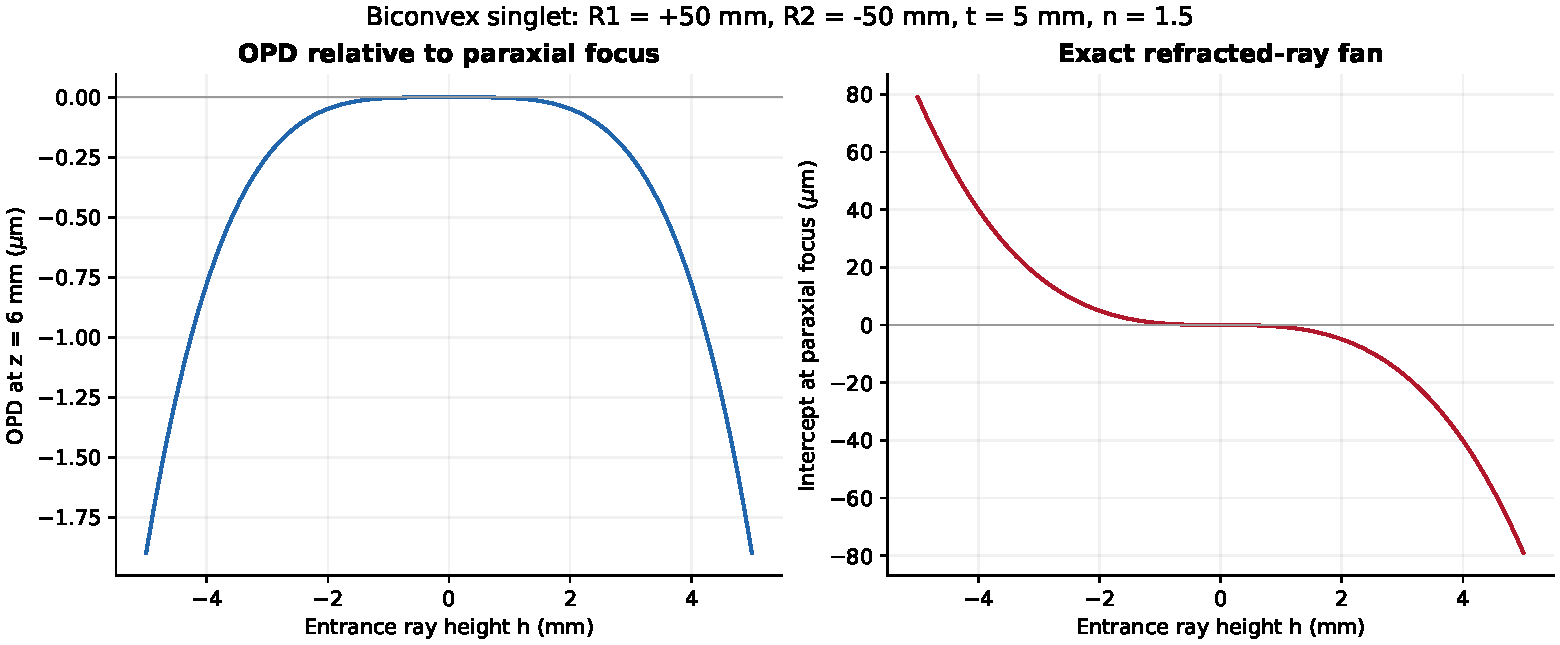
\includegraphics[width=\textwidth]{../figures/thick_singlet_checks.pdf}
 \caption{Exact ray and OPD checks for the finite singlet. The horizontal
 coordinate is entrance ray height. The comparison explicitly includes
 refraction at both surfaces and optical travel inside the glass.}
\end{figure}

\section{Checks that distinguish a model from a trustworthy calculation}
A useful ray tracer should pass checks with known consequences. A
plane-parallel plate returns the emerging ray parallel to the incident
ray in identical external media. A paraboloid returns zero on-axis
reference OPD in the ideal geometry. Rays near the axis approach the
paraxial matrix result. The eikonal gradient at a common output plane
agrees with actual minus ideal transverse optical momentum:
\begin{equation}
 \nabla_{\perp}W=n'(\bm s_{a,\perp}-\bm s_{i,\perp}).
\end{equation}
For the numerical singlet, a finite-difference derivative near the
ray launched at $h=3\,\mathrm{mm}$ gives
$\partial W/\partial y_6\simeq-3.4606372\times10^{-4}$, while the
independent difference of direction cosines gives
$-3.4606368\times10^{-4}$. Agreement checks signs, path accumulation,
and the common-plane mapping simultaneously.

Do not demand that the simple paraxial spot relation
$\Delta\bm x=(L/n')\nabla_\perp W$ reproduce every higher-order term
of an exact high-aperture ray trace. Exact propagation uses
$\bm x_f=\bm x_p+L\bm s_\perp/s_z$; the derivative of the factor
$1/s_z$ also matters beyond the leading paraxial approximation.

\chapter{Fitting measured data without losing its meaning}
\label{zc:fitting}

\section{From an integral to a matrix}
An instrument supplies samples $w_i$ at positions $(x_i,y_i)$, often
with missing values and nonuniform uncertainty. Choose $M$ retained
modes and form the design matrix
\begin{equation}
 A_{ij}=Z_j(\rho_i,\theta_i),\qquad
 \bm w\simeq A\bm c.
\end{equation}
For positive weights $q_i$, fit by minimizing
\begin{equation}
 J(\bm c)=\sum_iq_i\left[w_i-\sum_jA_{ij}c_j\right]^2
         =\lVert Q^{1/2}(\bm w-A\bm c)\rVert_2^2,
 \label{zc:weightedfit}
\end{equation}
where $Q=\operatorname{diag}(q_i)$. Equal-area pixels can use equal
area weights. A polar grid uniform in $\rho$ needs weights proportional
to $\rho$ away from the origin, or preferably a quadrature designed
for area integration. Independent measurements with known noise
variances $\sigma_i^2$ instead lead to statistical weights
$q_i=1/\sigma_i^2$ for a Gaussian-noise maximum-likelihood fit.

Area weighting and inverse-variance weighting answer different
questions. The former approximates a physical pupil RMS objective;
the latter extracts coefficients efficiently under a noise model.
They can be combined intentionally, but then the fitting objective
must be named. The RMS used to report optical performance can be
computed with a separate physical pupil measure after the fit.

Differentiating Eq.~\eqref{zc:weightedfit} gives the normal equations
\begin{equation}
 A^{\mathsf T}QA\,\bm c=A^{\mathsf T}Q\bm w.
 \label{zc:normalequations}
\end{equation}
They are helpful for understanding the geometry, but explicitly
inverting $A^{\mathsf T}QA$ is a poor default numerical method.
Forming this product squares the condition number of the weighted
design matrix and can amplify roundoff.

\section{QR and singular-value decomposition}
Set $B=Q^{1/2}A$ and $\bm y=Q^{1/2}\bm w$. A thin QR factorization
$B=UR$ has orthonormal columns in $U$ and an upper triangular matrix
$R$. For full column rank,
\begin{equation}
 R\bm c=U^{\mathsf T}\bm y.
\end{equation}
Solve this triangular system by back-substitution. There is no need
to compute $R^{-1}$ explicitly.

A singular-value decomposition is
\begin{equation}
 B=U\Sigma V^{\mathsf T},\qquad
 \Sigma=\operatorname{diag}(s_1,\ldots,s_r),\quad s_1\geq\cdots>0.
\end{equation}
It gives the least-squares solution
\begin{equation}
 \bm c=\sum_{k=1}^r
          \frac{\bm u_k^{\mathsf T}\bm y}{s_k}\bm v_k.
\end{equation}
Each $\bm v_k$ is a combination of modes. A tiny singular value means
that this combination produces very little signal on the measured
samples; noise divided by $s_k$ can then make its coefficient huge.
Truncating such directions stabilizes the fit but also declares them
unresolved. Report rank and the singular-value threshold.
The supplied code uses NumPy's documented least-squares interface,
which returns the rank and singular values~\cite{zc:numpylstsq}.

\section{Why masked projection is not least squares}
On a full, continuously sampled disk our normalized modes obey
$\langle Z_j,Z_k\rangle_D=\delta_{jk}$. After a central obstruction
or missing sector, their Gram matrix becomes
\begin{equation}
 G_{jk}=\langle Z_j,Z_k\rangle_{\mathrm{mask}},
\end{equation}
and generally $G\ne I$. Taking each masked dot product as a coefficient
gives $\bm b=G\bm c$ even for perfectly noiseless data in the model.
Thus each reported value includes contributions from other modes.
Least squares solves the coupled problem instead.

The numerical companion constructs a known combination of 28 modes
through $n=6$ and removes an obscured centre, a support strip, and a
sector. Correct weighted least squares recovers the coefficients to
about $10^{-16}\,\mu\mathrm m$ in that noiseless numerical example.
Treating normalized masked dot products as coefficients produces a
maximum error of approximately $0.0205\,\mu\mathrm m$.
This is a controlled demonstration of mode mixing, not a claim that
real metrology achieves machine-precision accuracy.

\section{Residuals, uncertainty, and the cost of adding modes}
After fitting, compute $r_i=w_i-(A\widehat{\bm c})_i$. Plot the
residual as a map. A single residual RMS cannot reveal whether the
remaining error is a scratch, a clipped edge, a periodic tool mark,
or a smooth omitted mode. Examine residual structure, sampling scale,
and repeated measurements.

If the noise vector has covariance $\Sigma_\epsilon$ and the fit is
linear, $\widehat{\bm c}=H\bm w$ for an estimator matrix $H$. Hence
\begin{equation}
 \operatorname{Cov}(\widehat{\bm c})=H\Sigma_\epsilon H^{\mathsf T}.
\end{equation}
When $Q=\Sigma_\epsilon^{-1}$ and the model has full column rank,
the algebraic covariance is
\begin{equation}
 \operatorname{Cov}(\widehat{\bm c})=(A^{\mathsf T}
             \Sigma_\epsilon^{-1}A)^{-1}.
\end{equation}
This identity explains the statistics; evaluate it through a stable
factorization, not an unnecessary explicit normal-matrix inverse.
For independent noise of unknown common standard deviation, a
residual estimate is $\widehat\sigma^2=\sum_i r_i^2/(N-r)$ with
fit rank $r$, provided the model is adequate and the samples are
independent. Correlated pixels reduce the effective information; simply
counting every pixel as independent understates uncertainty.

For a scalar full-disk RMS $\sigma=\sqrt{\bm c^{\mathsf T}P\bm c}$,
where $P$ selects the retained error coefficients, first-order error
propagation gives
\begin{equation}
 \operatorname{Var}(\sigma)\simeq
 \frac{(P\bm c)^{\mathsf T}\operatorname{Cov}(\bm c)(P\bm c)}
      {\sigma^2}.
\end{equation}
This linear approximation fails near zero RMS, where the norm is
nonlinear and the denominator vanishes. Monte Carlo propagation or an
appropriate confidence bound is then more useful.

Adding modes cannot increase the training residual in ordinary least
squares, but can fit noise and make coefficients unstable. Choose an
order using the spatial resolution, expected physics, singular values,
repeatability, and prediction on withheld data. A small change in pupil
edge location should not produce a large unsupported change in the
research conclusion. Repeat the fit over a reasonable range of orders
and report which conclusions are stable.

\section{Fitting slopes measured by a wavefront sensor}
A Shack--Hartmann sensor measures local ray directions through spot
displacements. If a lenslet has focal length $f_\ell$ and output index
$n'$, the local paraxial relation is
\begin{equation}
 \Delta x_\ell\simeq\frac{f_\ell}{n'}
                   \left\langle\partial_x W\right\rangle_\ell,
 \qquad
 \Delta y_\ell\simeq\frac{f_\ell}{n'}
                   \left\langle\partial_y W\right\rangle_\ell.
\end{equation}
The average is over a lenslet footprint with appropriate illumination
weighting. Build a design matrix from averaged derivatives of the
Zernikes, stack the two slope components, and solve the same weighted
least-squares problem. Point evaluation at lenslet centres is an
additional approximation for modes varying appreciably across a
lenslet.

Piston has zero derivative and is unobservable from slopes alone; its
column is identically zero. Remove it from the fit or impose a gauge
such as zero mean. Disconnected pupil regions can have additional
unobserved differential pistons. A numerical pseudoinverse selecting
zero for an unobserved quantity does not constitute a measurement of
that quantity. ESO's instrument documentation provides an example of
wavefront-sensor measurements used to guide mirror corrections
\cite{zc:esoSensor}.

\chapter{Changing pupils, coordinates, and illumination}
\label{zc:pupils}

\section{Rotating a wavefront without changing its strength}
Take one angular pair with coefficients $(a_c,a_s)$ multiplying
$N R_n^m\cos m\theta$ and $N R_n^m\sin m\theta$, $m>0$.
Physically rotate the pattern counterclockwise by $\alpha$ while
holding the axes fixed. The new map is
$W_{\mathrm{new}}(\rho,\theta)=W_{\mathrm{old}}(\rho,\theta-\alpha)$.
Expand both trigonometric functions:
\begin{align}
 \cos[m(\theta-\alpha)]
   &=\cos m\theta\cos m\alpha+\sin m\theta\sin m\alpha,\\
 \sin[m(\theta-\alpha)]
   &=\sin m\theta\cos m\alpha-\cos m\theta\sin m\alpha.
\end{align}
Collecting coefficients gives
\begin{equation}
 \begin{pmatrix}a_c'\\a_s'\end{pmatrix}=
 \begin{pmatrix}\cos m\alpha&-\sin m\alpha\\
                 \sin m\alpha&\cos m\alpha\end{pmatrix}
 \begin{pmatrix}a_c\\a_s\end{pmatrix}.
 \label{zc:rotation}
\end{equation}
The matrix preserves $a_c^2+a_s^2$. A rotation mixes members of an
angular pair, not different radial degrees. A passive rotation of the
coordinate axes uses the opposite angle. A reversal $Y\mapsto-Y$
leaves cosine modes unchanged and reverses the signs of sine modes.

For example, pure cosine astigmatism rotated through $45^\circ$ becomes
pure sine astigmatism because $m\alpha=90^\circ$. Pure cosine trefoil
rotated through $30^\circ$ similarly becomes pure sine trefoil. The
factor $m$ is why mode orientation cannot be read by treating every
pair like ordinary tilt.

\section{Changing the pupil radius mixes radial orders}
Suppose a measured physical wavefront was fitted on radius $a$, and
we now restrict it to the concentric radius $b=ka$ with $0<k<1$.
For the new normalized coordinate $\rho'=r/b$,
$\rho=k\rho'$. Even though the physical wavefront has not changed,
the polynomial arguments and the averaging domain have changed.

For pure defocus,
\begin{equation}
 c_2^0Z_2^0(k\rho')
 =k^2c_2^0Z_2^0(\rho')
       +\sqrt3(k^2-1)c_2^0.
\end{equation}
The new defocus coefficient scales by $k^2$, and the new pupil mean
changes. For pure primary spherical aberration, substitute $k\rho'$
into Eq.~\eqref{zc:sphericalpoly} and use the monomial identities:
\begin{align}
 c_4^{0\prime}&=k^4c_4^0,\\
 c_2^{0\prime}&=\sqrt{15}(k^4-k^2)c_4^0,\\
 c_0^{0\prime}&=\sqrt5(2k^4-3k^2+1)c_4^0.
 \label{zc:aperturescaling}
\end{align}
A pattern balanced on the original pupil is not generally balanced
on the smaller one. If the new observation can be refocused, remove
the newly generated focus component under the new pupil measure.
Scaling a measured coefficient by $k^n$ is therefore valid for the
highest radial degree in this example but misses induced lower modes.

Decentring also mixes orders and angular families. Expanding
$(X-\delta)^2+Y^2$ immediately produces a term linear in $X$; a
decentred focus pattern contains tilt and piston. Rather than relying
on a large table of transformation coefficients, evaluate the original
polynomials at transformed coordinates and refit on the desired pupil.
This method also handles combined translations, rotations, and scales,
provided the original map is known over the needed region. Extrapolating
beyond a measured aperture is an unsupported model prediction.

\section{Annular pupils: derive the simplest corrected mode}
Let a central obstruction remove $0\leq\rho<\epsilon$. The normalized
annular inner product is
\begin{equation}
 \langle f,g\rangle_A=
 \frac1{\pi(1-\epsilon^2)}\int_0^{2\pi}\int_\epsilon^1
                         fg\,\rho\,d\rho\,d\theta.
\end{equation}
The annular mean of $\rho^2$ is
\begin{equation}
 \frac{2}{1-\epsilon^2}\int_\epsilon^1\rho^3\,d\rho
          =\frac{1+\epsilon^2}{2}.
\end{equation}
Thus ordinary disk defocus has annular mean
$\langle Z_2^0,1\rangle_A=\sqrt3\epsilon^2$ and is no longer
orthogonal to piston. With $u=\rho^2$, the area measure is uniform
on $[\epsilon^2,1]$, whose variance is
$(1-\epsilon^2)^2/12$. Subtracting the mean and normalizing produces
\begin{equation}
 \boxed{Z_{2,A}^0=
 \frac{\sqrt3[2\rho^2-(1+\epsilon^2)]}{1-\epsilon^2}.}
 \label{zc:annulardefocus}
\end{equation}
This derivation illustrates the principle behind annular orthogonal
bases. Their coefficients are not interchangeable with coefficients
of ordinary disk polynomials restricted to an annulus.

Either representation can be useful. Ordinary disk functions retain
familiar shape labels and can be fitted together by least squares.
An orthonormal annular or numerically orthogonalized basis gives simple
RMS sums for that aperture. State which basis was used and preserve
the mask that defines it.

\section{Elliptical and grazing-incidence footprints}
For an ellipse with semiaxes $a_x,a_y$, use
$X=x/a_x$, $Y=y/a_y$ after aligning the axes. Its interior maps to a
unit disk. Since the area Jacobian is the constant $a_xa_y$, disk
Zernikes composed with this mapping are orthonormal for uniform
physical area on the ellipse. This is a coordinate construction; it
does not make the optical system rotationally symmetric. Physical
slopes have different factors $1/a_x$ and $1/a_y$, and optical
interpretations of ``defocus'' or ``astigmatism'' must account for them.

An oblique beam's footprint on a flat mirror is stretched along the
plane of incidence. At grazing incidence, let $\gamma$ be the angle
above the surface, so $i=\pi/2-\gamma$ and
\begin{equation}
 \delta W=-2nh\sin\gamma.
\end{equation}
The smaller OPD sensitivity per unit normal height does not mean that
surface accuracy becomes irrelevant. The footprint is long, the
mapping is anisotropic, angular errors still affect the image, and
very short wavelengths make small absolute path errors significant.
For curved grazing mirrors, incidence and pupil magnification vary
across the footprint; use Eq.~\eqref{zc:mirrorcoupling} or direct tracing.

\section{Amplitude, phase, coatings, and short wavelengths}
A pupil field is complex:
\begin{equation}
 P(x,y;\lambda_0)=A(x,y;\lambda_0)
   \exp\left[i\frac{2\pi W_{\mathrm{geom}}(x,y)}{\lambda_0}
                  +i\phi_{\mathrm{coat}}(x,y;\lambda_0)\right].
\end{equation}
The amplitude $A$ includes illumination, obscurations, transmission,
and reflectivity. A spatially varying coating phase acts like an
additional OPD
\begin{equation}
 W_{\mathrm{coat}}=\frac{\lambda_0}{2\pi}\phi_{\mathrm{coat}},
\end{equation}
after a continuous phase branch and a piston reference have been
chosen. A uniform reflection phase contributes piston; a nonuniform
one can contribute focus or higher modes. Near a phase jump, unwrapping
and amplitude zeros require particular care.

Multilayer reflectors used in EUV and X-ray optics are interference
structures; their complex reflected amplitude depends on wavelength,
angle, polarization, and layer design. The CXRO multilayer tutorial
provides a primary laboratory introduction to that interference
mechanism~\cite{zc:cxro}. In such systems, a surface sag fit alone does
not determine the image. Combine geometrical path, coating response,
and amplitude propagation. A scalar OPD can also be inadequate when
polarization components acquire substantially different phases or
directions; the appropriate field model then has vector components.

\chapter{From Zernike coefficients to images}
\label{zc:images}

\section{Why rays alone cannot predict the point image}
Rays describe local propagation directions and are powerful for
layout and aberration diagnosis. They do not by themselves describe
interference across a finite pupil. Even a zero-aberration mirror has
a finite diffraction pattern. A point-spread function (PSF) describes
the intensity produced by one ideal point object; the PSF is the bridge
from a wavefront map to an image.

For monochromatic, scalar, paraxial propagation near an ideal focal
plane, the complex amplitude has the Fourier-integral form
\begin{equation}
 U(\xi,\eta)=C\iint_{\mathcal P}A(x,y)
      \exp\left[i k_0W(x,y)
       -i\frac{2\pi n'}{\lambda_0 f}(x\xi+y\eta)\right]dx\,dy,
 \label{zc:psf}
\end{equation}
where $k_0=2\pi/\lambda_0$, $f$ is the relevant pupil-to-image
Fourier scale in this simplified model, and $C$ is a propagation
constant. The PSF is proportional to $|U|^2$ with a chosen energy
normalization. This form follows by expanding propagation distance
to quadratic order: the ideal converging pupil phase cancels the
pupil-dependent quadratic term, leaving a linear phase in image
coordinates and the residual $W$.

For an aplanatic high-numerical-aperture system, or when polarization
matters, Eq.~\eqref{zc:psf} must be replaced by the corresponding
vector diffraction integral and correct pupil apodization. The
coefficient table remains a description of a phase map, but the
propagation model must match the physical regime.

\section{Deriving the small-error Strehl relation}
At the ideal image origin, Eq.~\eqref{zc:psf} becomes the sum of
pupil phasors. For real nonnegative amplitude $A$, define the coherent
amplitude-weighted average
\begin{equation}
 \langle f\rangle_{A}=
          \frac{\int_{\mathcal P}A f\,dA}{\int_{\mathcal P}A\,dA}.
\end{equation}
Relative to the ideal image with the \emph{same amplitude pupil},
the normalized central intensity is
\begin{equation}
 S_{\mathrm{centre}}=\left|\left\langle
                        e^{ik_0W}\right\rangle_A\right|^2.
 \label{zc:exactcentralstrehl}
\end{equation}
This is evaluated at the specified image point. If tilt or defocus is
present, that point may not be the image maximum. State whether a
reported Strehl uses a fixed reference, a recentered image, or an
optimized focus.

Choose piston so $\langle W\rangle_A=0$. Expand the exponential:
\begin{equation}
 \left\langle e^{ik_0W}\right\rangle_A
       =1-\frac{k_0^2}{2}\langle W^2\rangle_A
           -\frac{ik_0^3}{6}\langle W^3\rangle_A+\cdots.
\end{equation}
Multiplying by the complex conjugate and retaining second order gives
\begin{equation}
 \boxed{S_{\mathrm{centre}}\simeq1-k_0^2\sigma_{W,A}^2.}
 \label{zc:strehlsecond}
\end{equation}
For weak aberrations the leading image degradation depends on phase
variance. A frequently useful extension is
\begin{equation}
 S\approx\exp[-(2\pi\sigma_W/\lambda_0)^2],
 \label{zc:marechal}
\end{equation}
usually called the extended Mar\'echal approximation. The exponential
matches the second-order expansion and is exact for the central
phasor average of a zero-mean Gaussian distribution of phase values
under the averaging measure. It is not a universal exact law for
deterministic aberrations. In particular, do not apply it blindly to
large phase excursions, sparse phase defects, amplitude errors, or
strongly obscured and polarization-dependent systems.

For a uniform full disk, $\sigma_W$ can be obtained from the
appropriate Zernike coefficient sum. For nonuniform amplitude, the
variance entering Eq.~\eqref{zc:strehlsecond} is weighted by $A$,
not automatically by intensity $A^2$. Geometrical image statistics,
detector photon weights, metrology likelihoods, and coherent focal
amplitude therefore need not use the same weights.

\section{A wavelength comparison and a caution about RMS}
An OPD of $30\,\mathrm{nm}$ RMS corresponds to phase RMS
$2\pi(30/633)=0.298$ radians at $633\,\mathrm{nm}$. The exponential
estimate is $S\simeq0.915$. At $13.5\,\mathrm{nm}$ the same OPD is
more than two waves RMS, far outside the weak-aberration regime.
The numerical exponential would be tiny, but treating that number as
a reliable image prediction would be unjustified; calculate the
complex pupil and its diffraction pattern directly.

For a target $S\geq0.8$ within the weak-error approximation,
\begin{equation}
 \sigma_W\lesssim\frac{\lambda_0}{2\pi}\sqrt{-\ln0.8}
                  \simeq0.0752\lambda_0.
\end{equation}
This estimate is close to the familiar ``about a fourteenth of a
wavelength RMS'' rule. At $13.5\,\mathrm{nm}$ it is roughly
$1.02\,\mathrm{nm}$ OPD RMS, or $0.51\,\mathrm{nm}$ normal-incidence
surface RMS for a single ideal mirror in vacuum if all other error
sources are absent. A system budget must allocate error among optics,
alignment, coatings, and time variation; it cannot assign the entire
system allowance independently to every element.

Equal RMS does not imply equal PSF structure. Coma displaces energy
asymmetrically; astigmatism changes image shape with focus; a localized
defect can create a broad halo. The Strehl approximation compresses
image quality into one quantity valid under specified conditions.
For research, inspect the PSF, encircled energy, and, where relevant,
the optical transfer function in addition to RMS.

\section{Peak-to-valley error and slope error}
For pure defocus $W=cZ_2^0$, the centre and edge values are
$-\sqrt3c$ and $+\sqrt3c$, so
\begin{equation}
 \mathrm{PV}_{\mathrm{defocus}}=2\sqrt3|c|.
\end{equation}
For pure balanced spherical aberration,
$W=c\sqrt5(6u^2-6u+1)$ with $u=\rho^2$. The stationary point
satisfies $12u-6=0$, hence $u=1/2$. The polynomial is $1$ at both
endpoints and $-1/2$ at $u=1/2$, giving
\begin{equation}
 \mathrm{PV}_{\mathrm{spherical}}=\frac32\sqrt5|c|.
\end{equation}
Both modes have RMS $|c|$, yet their PV-to-RMS ratios differ. For a
sum of modes there is no general rule that adds their individual PVs
in quadrature. Extremes must be found from the combined map, with
sampling fine enough to resolve them.

Slope also gives a different metric. A small high-spatial-frequency
error can have a large gradient even when its height RMS is modest.
For a one-dimensional illustrative ripple $W=b\cos(k_xx)$, its
height amplitude is $b$, whereas its slope amplitude is $|bk_x|$.
This is why an optical surface specification often needs both low-order
figure information and a spatial-frequency or slope description.
Low-order Zernike coefficients alone do not constrain roughness or
all scattered light.

\section{Using a Fourier transform in practice}
Build a uniformly sampled Cartesian pupil, set the complex amplitude
to zero outside the physical mask, evaluate the phase, and transform
the complex field. Zero padding interpolates the sampled image more
finely; it does not add pupil information or repair an undersampled
wavefront. Check that doubling the pupil sampling no longer changes
the observables of interest appreciably.

For a grid pitch $\Delta x$ and transform size $N$, the spatial-frequency
pitch is $\Delta\nu=1/(N\Delta x)$. In the paraxial model of
Eq.~\eqref{zc:psf}, the image-plane sampling is
\begin{equation}
 \Delta\xi=\frac{\lambda_0 f}{n'N\Delta x}.
\end{equation}
Keep the ideal and aberrated pupils on the same grid with the same
amplitude and total energy when comparing peaks. If one plot is
normalized to its own maximum, its apparent peak no longer shows
Strehl. For broadband incoherent imaging, combine intensities at the
proper wavelength-dependent image scales; do not add monochromatic
complex amplitudes unless the physical fields are mutually coherent.

\chapter{A reproducible computational laboratory}
\label{zc:lab}

\section{What to calculate before fitting an unknown optic}
Before interpreting experimental data, fit a map whose answer is known.
This separates questions about your implementation from questions about
the optic. The following complete Python example uses only NumPy and
the standard library. Coefficients and OPD values are in nanometres.
The radial formula is suitable for the modest degree used here; it is
not intended as a high-order production evaluator.

The quadrature samples $u=\rho^2$ by Gauss--Legendre integration on
$[0,1]$ and samples angle uniformly. Since
$\langle f\rangle_D=\int_0^1\langle f(\sqrt u,\theta)\rangle_\theta du$,
the weights sum to one. The code verifies full-disk orthonormality,
then fits a deliberately masked pupil. It retains the ordinary disk
polynomials and uses least squares for their coupled masked fit.

\begin{lstlisting}[language=Python,caption={A self-contained Zernike fitting experiment.}]
from math import factorial
import numpy as np
from numpy.polynomial.legendre import leggauss

def zernike(n, m, rho, theta):
    ell = abs(m)
    if n < 0 or ell > n or (n - ell) % 2:
        raise ValueError("Invalid (n, m)")
    rho = np.asarray(rho, dtype=float)
    radial = np.zeros_like(rho)
    for s in range((n - ell) // 2 + 1):
        factor = ((-1)**s * factorial(n - s) /
                  (factorial(s) *
                   factorial((n + ell)//2 - s) *
                   factorial((n - ell)//2 - s)))
        radial += factor * rho**(n - 2*s)
    if m == 0:
        return np.sqrt(n + 1) * radial
    angle = np.cos(m*theta) if m > 0 else np.sin(ell*theta)
    return np.sqrt(2*(n + 1)) * radial * angle

def disk_grid(nr=32, nt=96):
    u, wu = leggauss(nr)
    rho, theta = np.meshgrid(np.sqrt((u + 1)/2),
                             2*np.pi*np.arange(nt)/nt,
                             indexing="ij")
    q = np.broadcast_to(wu[:, None]/(2*nt), rho.shape)
    return rho.ravel(), theta.ravel(), q.ravel()

def fit(A, w, q):
    sw = np.sqrt(q)
    B = A * sw[:, None]
    c, _, rank, singular = np.linalg.lstsq(B, w*sw,
                                          rcond=None)
    residual = w - A @ c
    rms = np.sqrt(np.sum(q*residual**2)/np.sum(q))
    condition = singular[0]/singular[-1]
    return c, residual, rms, rank, condition

rho, theta, q = disk_grid()
modes = [(n, m) for n in range(7)
                for m in range(-n, n+1, 2)]
A = np.column_stack([zernike(n, m, rho, theta)
                     for n, m in modes])
gram = A.T @ (q[:, None] * A)
assert np.max(np.abs(gram - np.eye(len(modes)))) < 1e-11

truth = np.zeros(len(modes))
specified = {(0, 0): 20., (1, 1): -35., (2, 0): 80.,
             (2, -2): 42., (3, 1): -25., (4, 0): 60.,
             (6, 0): 8.}
for pair, value in specified.items():
    truth[modes.index(pair)] = value
w = A @ truth

x, y = rho*np.cos(theta), rho*np.sin(theta)
valid = ((rho > 0.25) & (np.abs(x) > 0.04)
         & ~((x > 0.3) & (y > 0.25)))
Am, wm, qm = A[valid], w[valid], q[valid]
c, residual, rms, rank, condition = fit(Am, wm, qm)
assert rank == len(modes)
assert np.max(np.abs(c - truth)) < 1e-8
print("rank, condition, residual RMS [nm]:",
      rank, condition, rms)

# This next expression is deliberately wrong for the masked pupil.
naive = Am.T @ (qm*wm) / qm.sum()
print("wrong masked projection error [nm]:",
      np.max(np.abs(naive - truth)))

# An optional noise experiment; area weights stay area weights.
rng = np.random.default_rng(7)
noisy = wm + rng.normal(0., 2., size=wm.size)
cn, rn, rmsn, rankn, condn = fit(Am, noisy, qm)
print("noisy fit residual RMS [nm]:", rmsn)
for pair in specified:
    j = modes.index(pair)
    print(pair, "true, recovered [nm]:", truth[j], cn[j])
\end{lstlisting}

The random seed makes the final experiment repeatable for a given
numerical implementation. Its $2\,\mathrm{nm}$ sample noise is an
invented teaching input, not an instrument specification. The area
weights approximate the masked pupil norm; they are not being claimed
as an optimal likelihood weighting for that synthetic noise model.
Notice that the printed rank is checked independently of a small
residual. An underdetermined fit can also have zero residual.

\section{Extending the experiment deliberately}
First change the known coefficient of one mode and verify that the
recovered value follows it. Then remove a larger pupil sector and
watch the condition number and coefficient noise sensitivity. Next
add a mode of degree higher than the fit includes; the residual should
show spatial structure. Finally perturb the assumed pupil centre and
radius to observe how geometry errors redistribute coefficients.

To connect the code with a real map, replace the synthetic $w$ and
sample coordinates by calibrated measurements, keep explicit units,
and build the physical mask. Preserve the raw measurement and its
original metadata. Phase in radians must be converted by
$W=\lambda_0\phi/(2\pi)$ only after any necessary phase unwrapping;
a wrapped phase map does not describe a continuous OPD by direct
pointwise multiplication alone.

The file \texttt{../verify\_optics.py} supplied alongside these books
contains additional symbolic checks, the exact spherical mirror trace,
the finite-thickness singlet trace, and figure generation. Its output
is recorded in \texttt{../numerical\_checks.txt}. The code distinguishes
surface-footprint, entrance-labelled, and output-plane quantities in
its comments and report. Use those distinctions when reproducing a
coefficient table.

\begin{figure}[p]
 \centering
 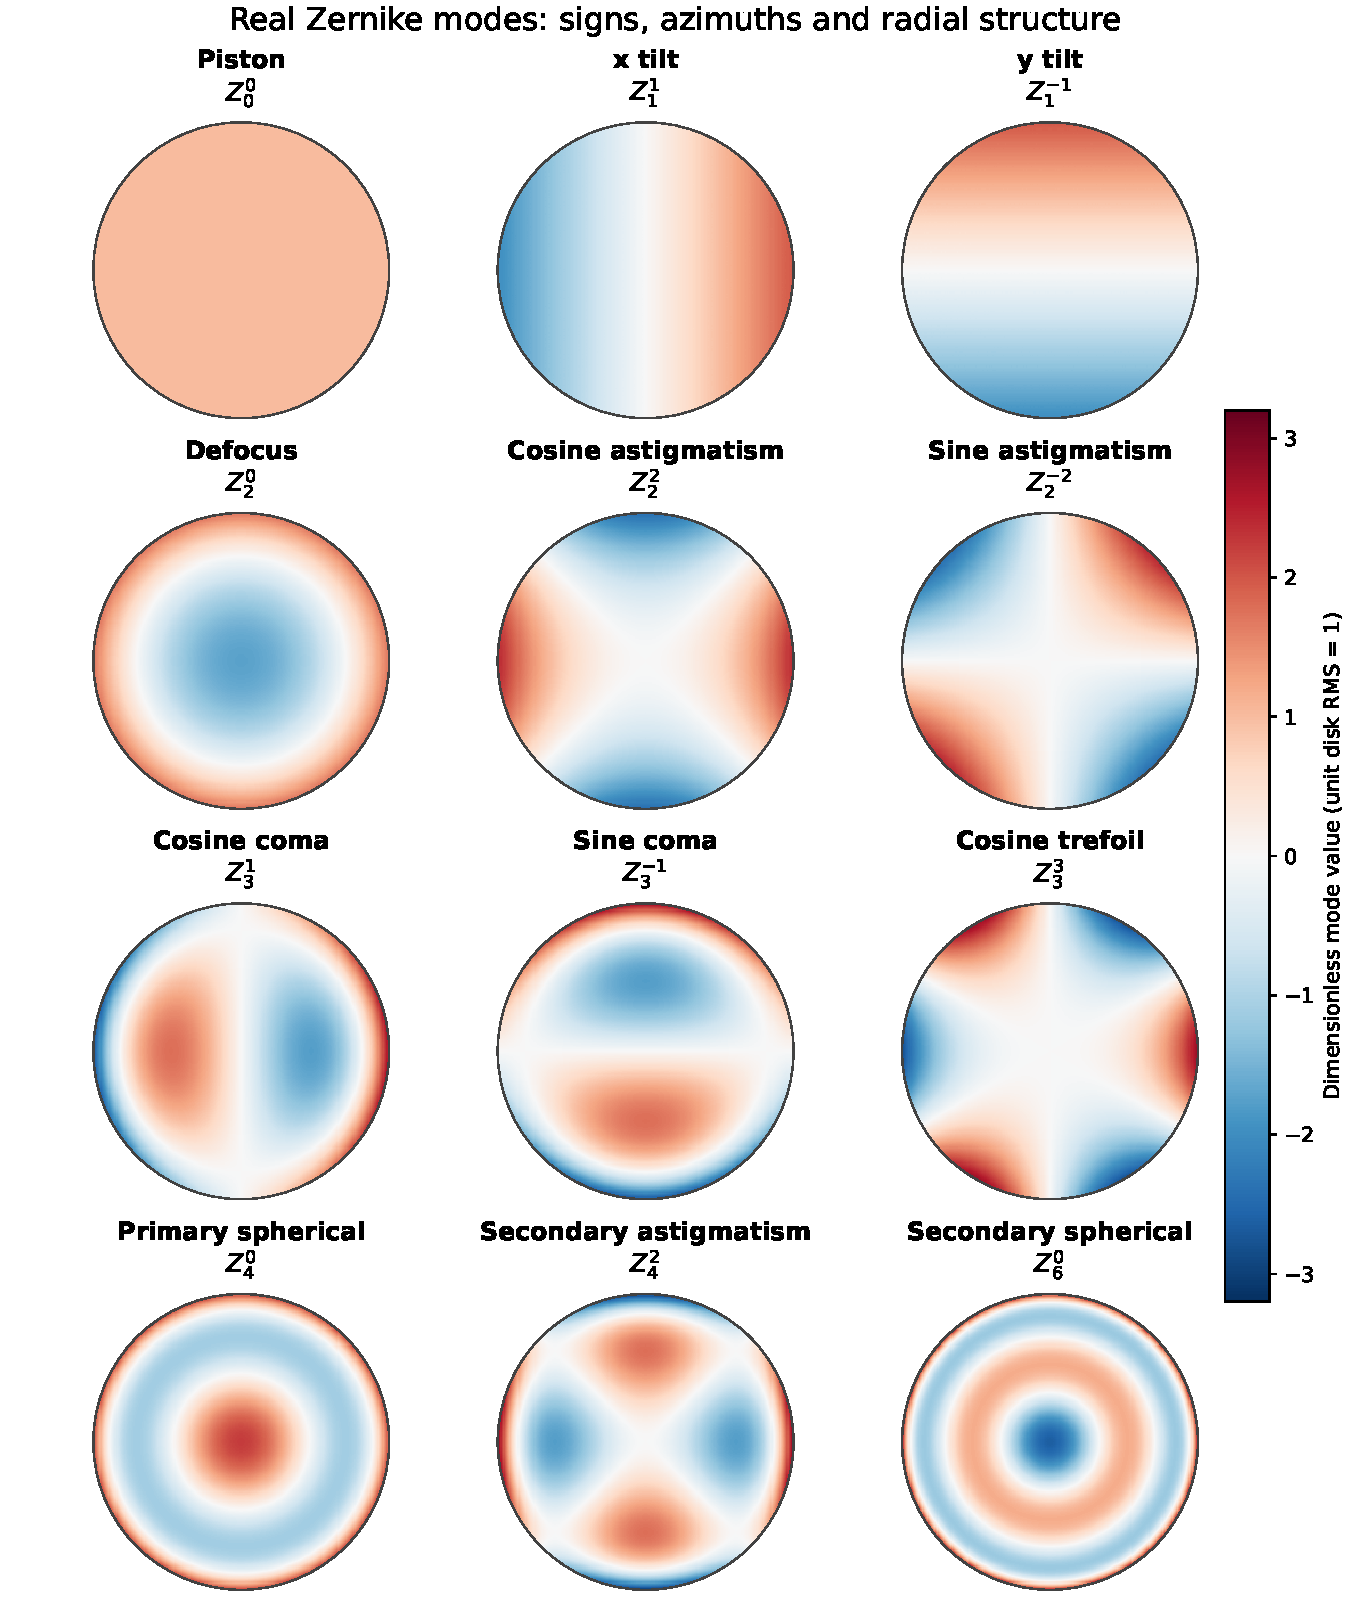
\includegraphics[width=0.93\textwidth,height=0.84\textheight,keepaspectratio]
                 {../figures/zernike_mode_atlas.pdf}
 \caption{Selected real disk-RMS-normalized modes. Colour represents
 polynomial value, not an assigned physical height. A coefficient
 with length units supplies that scale. The mode formula and colour
 scale must both be read when comparing patterns.}
\end{figure}

\chapter{Planning a first research investigation}
\label{zc:research}

\section{A question that can be answered with coefficients}
A productive starting question is concrete: ``For a specified mirror
aperture, object direction, wavelength, and image plane, how much does
a particular surface change reduce residual OPD and improve the image?''
The answer requires a nominal model, a change, a comparison procedure,
and a performance metric. A list of small coefficients by itself does
not show that an optical system satisfies its purpose.

Begin with a nominal prescription and an analytic limiting case.
For an on-axis paraboloid, verify equal path; for a singlet, verify
the paraxial focal lengths. Record the common reference surface and
pupil map. Increase aperture or field gradually so you can see when
the leading-order formulas stop matching the exact trace. This process
turns aberration theory into a controlled approximation whose error
can be measured.

\section{Linear sensitivity and design changes}
Let $p_k$ be adjustable prescription parameters: curvature, conic
constant, an aspheric coefficient, decentre, or an actuator command.
At a nominal design compute coefficients $\bm c(\bm p)$. For small
parameter changes,
\begin{equation}
 \bm c(\bm p+\delta\bm p)\simeq\bm c(\bm p)+J\delta\bm p,
 \qquad J_{jk}=\frac{\partial c_j}{\partial p_k}.
\end{equation}
A symmetric finite difference estimates a column:
\begin{equation}
 J_{jk}\simeq\frac{c_j(\bm p+\Delta p_k\bm e_k)
                       -c_j(\bm p-\Delta p_k\bm e_k)}{2\Delta p_k}.
\end{equation}
Choose a step small enough to describe local response but large enough
to exceed numerical noise; check the result when the step is halved
or doubled. Keep pupil, field, reference, and removed-term policy
consistent while taking these differences.

One local correction solves $J\delta\bm p\simeq-\bm c$ for the
selected error coefficients. Use a weighted and possibly regularized
least-squares solve. For example,
\begin{equation}
 \min_{\delta\bm p}
   \lVert L(\bm c+J\delta\bm p)\rVert_2^2
      +\alpha\lVert R\delta\bm p\rVert_2^2.
\end{equation}
Here $L$ scales optical priorities, $R$ scales the cost of changes,
and $\alpha$ controls that tradeoff. Bounds can enforce manufacturing
or actuator limits. Afterwards, recompute the full nonlinear optical
model. A small residual in the linear model is a proposed step, not
proof of the final physical performance.

If two parameters have nearly identical sensitivity columns, their
individual values cannot be determined reliably from those coefficients
alone. Add another field, wavelength, measurement geometry, or
independent surface measurement to distinguish them. This is an
identifiability problem, not a failure that can be repaired merely by
printing more digits.

\section{A published case: the Hubble primary-mirror test}
NASA's 1990 optical-failure investigation described a roughly
$1.3\,\mathrm{mm}$ spacing error in a lens of the reflective null
corrector used to test the Hubble primary mirror. The report estimated
about $0.4$ wave RMS of third-order spherical wavefront aberration at
$632.8\,\mathrm{nm}$ from the as-built mirror information
\cite{zc:hubble}. A null corrector supplies the intended comparison
wave for an aspheric test; an error in that comparison can make a
precisely manufactured wrong shape appear to pass the test.

Convert the stated wavefront RMS to length and phase:
\begin{align}
 \sigma_W&=0.4(632.8\,\mathrm{nm})=253.12\,\mathrm{nm},\\
 \sigma_\phi&=2\pi(0.4)=2.5133\,\mathrm{rad}.
\end{align}
This phase RMS is not small. Therefore the exponential small-error
Strehl approximation is not a reliable way to reconstruct the actual
telescope image from this one number. Neither can we simply declare
$c_4^0=253.12\,\mathrm{nm}$ in this book's convention: the historical
test, telescope pupil, reference, and normalization must first be
matched to our full-disk definition.

The methodological lesson for a new mirror project is to test the
reference as carefully as the optic. A self-consistent measurement
against one reference can preserve that reference's systematic error.
An independent test geometry or independently calibrated reference
helps distinguish true surface error from an error in the metrology
model. Numerical recovery of synthetic coefficients checks software;
it does not validate the physical reference used by an experiment.

\section{What belongs in a research notebook}
For each coefficient table, save the physical prescription or measured
map, wavelength and index data, object field, stop and pupil definition,
coordinate axes, unit conversions, actual-minus-ideal sign, reference
focus, mask, weighting, fitted mode list, and removed terms. Save the
residual map, fit rank, and convergence checks beside the table.
Include a reconstructed map and at least one image or ray diagnostic
whose coordinate scales are labelled.

Compare alternative designs at the same physical requirement. Allowing
one design to refocus at every wavelength while forcing another onto
a common detector biases the comparison. Similarly, excluding a bad
edge region changes the aperture and throughput as well as the RMS.
Such choices can be legitimate, but they belong in the experimental
question and must appear in the reported result.

For a first study, a useful deliverable is a short reproducible report
with an analytic leading-order estimate, an exact ray trace, an OPD
fit, a residual map, a diffraction calculation where applicable, and
a sensitivity study. The goal is not to make every coefficient zero.
It is to understand which physical changes improve the required
performance, how robust that improvement is, and what the model
still leaves unresolved.

\chapter{Exercises with detailed worked solutions}
\label{zc:exercises}

\section{How to use the problems}
Attempt each problem before reading its solution. Keep a units column
in numerical work and write the pupil and reference before every
coefficient calculation. The problems progress from integral practice
to design interpretation. Research extensions deliberately admit more
than one sensible modelling choice, but a justified choice is part
of the answer.

\subsection*{Problem 1: area averages and an incorrect radial average}
Find the disk mean and piston-removed RMS of $W=B\rho^2$. Explain why
sampling 100 equally spaced radii with equal weights gives a different
answer even as the number of radial samples grows.

\paragraph{Solution.}
Using $\langle\rho^2\rangle_D=1/2$ and
$\langle\rho^4\rangle_D=1/3$,
\begin{equation}
 \overline W=\frac B2,\qquad
 \sigma^2=B^2\left(\frac13-\frac14\right)=\frac{B^2}{12}.
\end{equation}
Thus $\sigma=|B|/(2\sqrt3)$, consistent with the defocus coefficient.
Equal radial weights approach an integral in $d\rho$, not in
$2\rho\,d\rho$, and return mean $B/3$. To represent area, sample
$u=\rho^2$ uniformly or apply appropriate area weights. Increasing
the number of samples does not repair the wrong measure.

\subsection*{Problem 2: build a secondary radial polynomial}
Construct $R_4^2$ using $\rho^4-\beta\rho^2$, with orthogonality to
$\rho^2$ under the radial measure $\rho\,d\rho$ and boundary value
$R_4^2(1)=1$.

\paragraph{Solution.}
The orthogonality condition is
\begin{equation}
 \int_0^1(\rho^4-\beta\rho^2)\rho^2\rho\,d\rho
      =\frac18-\frac\beta6=0,
\end{equation}
so $\beta=3/4$. At the edge the unscaled polynomial is $1/4$;
multiply by four to obtain $R_4^2=4\rho^4-3\rho^2$.
Multiplication by $\sqrt{10}\cos2\theta$ or
$\sqrt{10}\sin2\theta$ gives the two RMS-normalized real modes.

\subsection*{Problem 3: recover coefficients from a Cartesian map}
On a unit disk, let
$W=(10+12X-8Y+6X^2-6Y^2)\,\mathrm{nm}$. Find all nonzero
coefficients and the piston-removed RMS.

\paragraph{Solution.}
Use $Z_0^0=1$, $Z_1^1=2X$, $Z_1^{-1}=2Y$, and
$Z_2^2=\sqrt6(X^2-Y^2)$. The coefficients are
\begin{equation}
 c_0^0=10,\quad c_1^1=6,\quad c_1^{-1}=-4,\quad
 c_2^2=\frac6{\sqrt6}=\sqrt6,
\end{equation}
all in nanometres. The RMS after piston removal is
$\sqrt{36+16+6}=\sqrt{58}=7.616\,\mathrm{nm}$.
If pointing is also removed, only astigmatism remains and the RMS is
$\sqrt6=2.449\,\mathrm{nm}$. Both answers are valid for different
removed-term policies.

\subsection*{Problem 4: balance quartic and sixth-power error}
Starting from $W=A\rho^4+B\rho^6$, find the added polynomial
$D\rho^2+P$ that makes both the disk mean and the defocus coefficient
zero. Derive the remaining RMS.

\paragraph{Solution.}
Equation~\eqref{zc:quarticsixth} gives
$c_2^0=(D+A)/(2\sqrt3)+9B/(20\sqrt3)$. Setting this to zero yields
$D=-A-9B/10$. The mean is $P+D/2+A/3+B/4$, so
\begin{equation}
 P=\frac A6+\frac B5.
\end{equation}
The remaining two coefficients are unchanged by piston and defocus:
$c_4^0=(A/6+B/4)/\sqrt5$ and $c_6^0=B/(20\sqrt7)$. Hence
\begin{equation}
 \sigma_{\mathrm{balanced}}=
 \sqrt{\frac{(A/6+B/4)^2}{5}+\frac{B^2}{2800}}.
\end{equation}
Notice that $B$ changes the best defocus and the primary spherical
coefficient. It cannot be treated as an isolated secondary spherical
mode unless those lower-order changes are compensated.

\subsection*{Problem 5: mirror height and correction sign}
A mirror in air has positive normal toward the incident beam. Its
measured reflected OPD includes $c_3^1=+60\,\mathrm{nm}$. Under
normal-incidence, small-deformation assumptions, what surface
coefficient produced it, and what added surface coefficient removes it?

\paragraph{Solution.}
Since $c_3^1=-2b_3^1$, the inferred departure is
$b_3^1=-30\,\mathrm{nm}$. The correction must add
$+30\,\mathrm{nm}$ in the same normalized surface mode. It creates
$-60\,\mathrm{nm}$ of OPD and cancels the measured term. A physical
actuator solution must still account for influence functions and the
actual pupil mapping.

\subsection*{Problem 6: compare normal and grazing incidence}
A normal surface-height error is $10\,\mathrm{nm}$ in vacuum.
Find its OPD magnitude at normal incidence, at $i=60^\circ$ from the
normal, and at a grazing angle $\gamma=2^\circ$ above the surface.

\paragraph{Solution.}
Use $|\delta W|=2|h|\cos i=2|h|\sin\gamma$ as appropriate.
The three magnitudes are $20\,\mathrm{nm}$, $10\,\mathrm{nm}$,
and $20\sin2^\circ=0.6980\,\mathrm{nm}$. The signed values are
negative for positive height in our convention. At short wavelength,
even the last OPD can be significant. These are local normal-height
sensitivities, not complete imaging predictions.

\subsection*{Problem 7: infer a lens thickness coefficient}
A weak element in air has index $1.60$ and induced OPD coefficient
$c_2^{-2}=18\,\mathrm{nm}$. Find the corresponding thickness
coefficient. If the index becomes $1.58$ at a second wavelength,
what is that coefficient in OPD length units there?

\paragraph{Solution.}
The thickness coefficient is $b=18/0.60=30\,\mathrm{nm}$.
At the second wavelength the OPD coefficient is
$0.58(30)=17.4\,\mathrm{nm}$. To quote it in waves, divide by the
second vacuum wavelength in nanometres. The index change alone is
insufficient to determine the number of waves.

\subsection*{Problem 8: translate a focus coefficient into a distance}
At a pupil of radius $a=10\,\mathrm{mm}$ in air, the reference focus
is $L=200\,\mathrm{mm}$ downstream and the OPD defocus coefficient
is $c_2^0=+50\,\mathrm{nm}$. Estimate the reference-focus shift
needed to remove this coefficient.

\paragraph{Solution.}
Convert $50\,\mathrm{nm}=5.0\times10^{-5}\,\mathrm{mm}$.
Equation~\eqref{zc:focusshift} gives
\begin{equation}
 \delta L=\frac{4\sqrt3(200)^2}{(10)^2}
                       (5.0\times10^{-5})\,\mathrm{mm}
           =0.13856\,\mathrm{mm}.
\end{equation}
The new reference lies farther downstream. Holding the actual
wavefront fixed while increasing $L$ increases the ideal quadratic
eikonal, thereby decreasing the positive residual focus coefficient.

\subsection*{Problem 9: interpret a rotated astigmatism pair}
A map has $c_2^2=30\,\mathrm{nm}$ and
$c_2^{-2}=40\,\mathrm{nm}$. Find its pair RMS and orientation.
Then physically rotate the map by $15^\circ$ and find the new pair.

\paragraph{Solution.}
The pair RMS is $50\,\mathrm{nm}$ and
$\psi=\tfrac12\operatorname{atan2}(40,30)=26.565^\circ$ modulo
$180^\circ$. The coefficient rotation angle is $2(15^\circ)=30^\circ$:
\begin{align}
 a_c'&=30\cos30^\circ-40\sin30^\circ=5.981\,\mathrm{nm},\\
 a_s'&=30\sin30^\circ+40\cos30^\circ=49.641\,\mathrm{nm}.
\end{align}
The new pair still has norm $50\,\mathrm{nm}$ and its orientation
has increased to $41.565^\circ$.

\subsection*{Problem 10: stop down a balanced spherical mode}
A full pupil has only $c_4^0=100\,\mathrm{nm}$. Restrict the radius
by $k=1/2$. Find the new non-piston coefficients before and after
refocusing.

\paragraph{Solution.}
Equation~\eqref{zc:aperturescaling} gives
$c_4^{0\prime}=100/16=6.25\,\mathrm{nm}$ and
\begin{equation}
 c_2^{0\prime}=100\sqrt{15}\left(\frac1{16}-\frac14\right)
                  =-72.618\,\mathrm{nm}.
\end{equation}
The piston also changes but is not needed for the requested RMS.
Before refocusing the error is dominated by the new defocus component.
After refocusing the remaining RMS is $6.25\,\mathrm{nm}$ in this
idealized case. Stopping down reduces the highest-power error strongly,
but the original full-pupil balance must be reconsidered.

\subsection*{Problem 11: an annulus makes a familiar mode nonzero-mean}
For central obstruction ratio $\epsilon=0.30$, calculate the annular
mean of ordinary disk defocus $Z_2^0$. Give an annular unit-RMS
defocus mode.

\paragraph{Solution.}
The mean is $\sqrt3\epsilon^2=0.155885$, which is nonzero.
Using Eq.~\eqref{zc:annulardefocus},
\begin{equation}
 Z_{2,A}^0=\frac{\sqrt3(2\rho^2-1.09)}{0.91},
 \qquad0.30\leq\rho\leq1.
\end{equation}
It has zero annular mean and unit annular RMS. Its normalization
depends on the obstruction ratio; changing the obstruction changes
the basis.

\subsection*{Problem 12: distinguish an index from a coefficient}
One program exports $b=0.12\,\mu\mathrm m$ multiplying
$F=6\rho^4-6\rho^2+1$. Another uses this book's normalized
$Z_4^0$. Find the second coefficient and the piston-removed RMS.

\paragraph{Solution.}
Because $Z_4^0=\sqrt5F$,
$bF=(b/\sqrt5)Z_4^0$. The coefficient is
$c_4^0=0.12/\sqrt5=0.053666\,\mu\mathrm m$.
For this isolated normalized non-piston mode, its RMS is the same
magnitude. Merely copying $0.12$ into the other program would multiply
the represented wavefront by $\sqrt5$.

\subsection*{Problem 13: identify an unobservable quantity}
You measure exact $x$ and $y$ wavefront slopes everywhere on a connected
pupil. Can you determine piston? What changes if the pupil has two
disconnected illuminated regions and no relative-phase measurement?

\paragraph{Solution.}
Adding a constant to $W$ leaves both derivatives unchanged, so absolute
piston is unobservable. On two disconnected regions, an independent
constant can be added to each while preserving all measured slopes.
Their difference is differential piston and affects interference when
the fields combine, but the stated measurements do not determine it.
Any fit that reports a unique value has imposed an additional constraint
or prior; it has not extracted that value from the slopes alone.

\subsection*{Problem 14: derive a leading spherical-mirror ray error}
For the mirror at Gaussian focus $f=R/2$, use the leading plane OPD
$W(x)=-x^4/(4R^3)$ to estimate the transverse ray error in air.
Explain why the same operation on the sixth-order OPD is not an exact
fifth-order ray calculation.

\paragraph{Solution.}
The gradient is $dW/dx=-x^3/R^3$. The paraxial relation gives
\begin{equation}
 \Delta x\simeq f\frac{dW}{dx}=-\frac{x^3}{2R^2}.
\end{equation}
It is cubic in pupil coordinate: the primary wave error is quartic,
while the corresponding ray error is third order. At higher accuracy,
ray propagation involves $s_x/s_z$, not just $s_x$. The ideal ray
is already inclined away from the axis, so linearizing this ratio
introduces additional powers. Reference-plane and pupil-coordinate
mapping must also be retained consistently.

\subsection*{Problem 15: a small-error image estimate}
A uniformly illuminated circular pupil has nonzero retained error
coefficients $20,15,-10\,\mathrm{nm}$ after allowed pointing and
focus adjustments. At $\lambda_0=550\,\mathrm{nm}$ estimate the
RMS and Strehl, and state what is missing from that estimate.

\paragraph{Solution.}
The RMS is $\sqrt{400+225+100}=26.926\,\mathrm{nm}$.
The phase RMS is $2\pi(26.926/550)=0.3076$ radians, so
$S\approx\exp(-0.3076^2)=0.910$.
This omits any unmodelled residual, amplitude variation, polarization
effects, and mismatch between the simplified propagation and the
actual system. It also does not describe how energy is distributed
around the peak. Calculate the PSF if those details matter.

\subsection*{Problem 16: distinguish two planes in a mirror calculation}
Two calculations of the same sphere return sixth-power coefficients
$1/(8R^5)$ and $9/(8R^5)$ in OPD length per sixth power of radius.
Both use the same actual-minus-ideal sign. Is one necessarily wrong?

\paragraph{Solution.}
No. The first can describe the common-surface optical path function
labelled by mirror footprint radius $r$, and the second the eikonal
difference on the virtual vertex plane labelled by intercept $x$.
The two points and their phase propagation differ, and
$x=r+r^3/R^2+\cdots$. Require the comparison surface, coordinate map,
and reference eikonal before comparing the series. The leading quartic
agreement alone is not sufficient to identify the higher-order
convention.

\subsection*{Problem 17: test whether fitting more modes helps}
You fit experimental data through radial degrees 4, 6, and 8. Training
RMS decreases at every step, but the degree-8 coefficients change
greatly when one small pupil sector is removed. What should you do?

\paragraph{Solution.}
Inspect singular values, parameter covariance or repeated-data
variability, and the spatial residual. The highest-order combinations
may be weakly constrained or absorbing noise and a mask-edge error.
Use held-out data or independent repeated maps to compare predictive
quality. Check pupil registration and sampling before increasing order
again. Retain an order justified by resolution and stability, or use
explicit regularization and report it. The training residual alone
does not establish that the extra fitted structure is physical.

\subsection*{Problem 18: a first independent design project}
Design a computational study comparing a spherical and paraboloidal
mirror with the same vertex radius, aperture, axial plane-wave input,
and available focus adjustment. Specify the quantities you will plot
and the checks that would make the comparison credible.

\paragraph{Worked research outline.}
Start from $z_s=R-\sqrt{R^2-r^2}$ and $z_p=r^2/(2R)$.
Verify exact constant path for the paraboloid and the quartic leading
term for the sphere. Trace reflected rays and calculate common-plane
OPD for both, preserving the ray-to-pupil map. Plot axial ray crossings,
transverse intercepts, fixed-focus OPD, balanced OPD, and radial
coefficients against aperture ratio $a/R$.

Find best phase-variance focus by an actual one-parameter search of
the reference location, and compare it with the paraxial prediction.
For a chosen wavelength, compute diffraction images on the same
normalized energy scale and compare peak, encircled energy, and shape.
Repeat with finer ray or pupil sampling and a higher fit order until
the reported metrics converge. Then add a small field angle and
observe that the paraboloid's on-axis advantage does not eliminate
off-axis aberrations. A useful report explains where each analytic
approximation works, where it fails, and how the result depends on
allowed refocusing and aperture.

\chapter*{Notation and formula reference}
\addcontentsline{toc}{chapter}{Notation and formula reference}
\begin{longtable}{@{}p{0.22\textwidth}p{0.71\textwidth}@{}}
\toprule Symbol or expression & Meaning and condition\\\midrule\endfirsthead
\toprule Symbol or expression & Meaning and condition\\\midrule\endhead
$a$ & Physical radius of the pupil used to normalize coordinates.\\
$\rho,\theta$ & Dimensionless pupil radius and counterclockwise polar angle.\\
$z,h$ & Surface sag and departure; positive direction must be stated.\\
$S,W$ & Eikonal in optical-length units, and actual-minus-ideal eikonal.\\
$\lambda_0,k_0$ & Vacuum wavelength and $2\pi/\lambda_0$.\\
$n,m$ in $Z_n^m$ & Radial degree and signed angular label;
these are distinct from refractive index, also often written $n$.\\
$m>0,m<0$ & Cosine and sine respectively in this book's real basis.\\
$c_n^m,b_n^m$ & OPD coefficients and surface or thickness coefficients,
respectively; all carry length units unless stated in waves.\\
$c_n^m=\langle W,Z_n^m\rangle_D$ & Projection on a full uniform disk;
masked data generally require a coupled fit.\\
$\sigma_W^2=\sum'c_j^2$ & Full-disk orthonormal RMS, with the prime excluding
piston and any other explicitly removed modes; add unfitted residual power.\\
$\delta W=-2nh\cos i$ & First-order mirror sensitivity for positive
normal height toward the incident medium.\\
$\delta W=(n_g-n_e)\delta t$ & Thin, nearly axial transmitting thickness
error replacing external medium.\\
$\nabla_\perp W/n'$ & Actual-minus-ideal transverse direction cosine on
a common output plane.\\
$\Delta\bm x\simeq(L/n')\nabla_\perp W$ & Forward paraxial transverse
ray displacement at propagation distance $L$.\\
$S\approx e^{-(2\pi\sigma_W/\lambda_0)^2}$ & Weak-aberration image estimate
with the stated pupil and image-reference conditions.\\
\bottomrule
\end{longtable}

\begin{thebibliography}{99}
\raggedright
\addcontentsline{toc}{chapter}{References and further study}
\bibitem{greivenkamp502}
John E. Greivenkamp, \emph{OPTI 502: Optical Design and Instrumentation I},
University of Arizona, course notes and worked instructional material.
\url{https://wp.optics.arizona.edu/jgreivenkamp/classes/opti-502/}.
A route to further study of geometrical optics, pupils, paraxial
ray tracing, and optical materials.

\bibitem{zc:wyant}
James C. Wyant and Katherine Creath, ``Basic Wavefront Aberration Theory
for Optical Metrology,'' in \emph{Applied Optics and Optical Engineering},
Vol. XI, Academic Press, 1992; author-hosted Zernike excerpt.
\url{https://wp.optics.arizona.edu/jcwyant/wp-content/uploads/sites/13/2016/08/Zernikes.pdf}.
Consult its stated normalization and signs before converting numbers.

\bibitem{zc:dlmfRodrigues}
NIST Digital Library of Mathematical Functions, Chapter 18,
\S18.5, ``Explicit Representations,'' especially the Jacobi Rodrigues
formula and finite series.
\url{https://dlmf.nist.gov/18.5}.
Related normalization and orthogonality conventions are in
\url{https://dlmf.nist.gov/18.3}.
The disk-specific construction and integration steps are developed
explicitly in this textbook.

\bibitem{zc:numpylstsq}
NumPy documentation, \texttt{numpy.linalg.lstsq}.
\url{https://numpy.org/doc/stable/reference/generated/numpy.linalg.lstsq.html}.
Documents least-squares outputs, numerical rank, singular values,
and the cutoff parameter used in the computational example.

\bibitem{zc:esoSensor}
European Southern Observatory, \emph{EFOSC2 User's Manual}, version 4.2,
discussion of image analysis and active-optics wavefront correction.
\url{https://www.eso.org/sci/facilities/lasilla/instruments/efosc/doc/manual/EFOSC2manual_v4.2.pdf}.

\bibitem{zc:cxro}
Center for X-Ray Optics, Lawrence Berkeley National Laboratory,
multilayer mirror tutorial.
\url{https://henke.lbl.gov/multilayer/mltutor.html}.
Laboratory introduction to coherent addition of reflections in
short-wavelength multilayer coatings.

\bibitem{zc:hubble}
NASA, \emph{The Hubble Space Telescope Optical Systems Failure Report},
NASA TM-103443, 1990, NASA Technical Reports Server record 19910003124.
\url{https://ntrs.nasa.gov/citations/19910003124}.
Historical primary investigation used for the metrology case study;
its error descriptions must be read with its original test conventions.
\end{thebibliography}
